% ---------------------------------------------------------------
% Preamble
% ---------------------------------------------------------------
%\documentclass[a4paper,fleqn,longmktitle]{cas-sc}
\documentclass[a4paper,fleqn]{cas-dc}
%\documentclass[a4paper]{cas-dc}
%\documentclass[a4paper]{cas-sc}
% ---------------------------------------------------------------
% Make margins bigger to fit annotations. Use 1, 2 and 3. TO be removed later
%\paperwidth=\dimexpr \paperwidth + 6cm\relax
%\oddsidemargin=\dimexpr\oddsidemargin + 3cm\relax
%\evensidemargin=\dimexpr\evensidemargin + 3cm\relax
%\marginparwidth=\dimexpr \marginparwidth + 3cm\relax
% -------------------------------------------------------------------- 
% Packages
% --------------------------------------------------------------------
% Figure packages
\usepackage{graphicx,float}
\restylefloat{table}
\usepackage{adjustbox}
% Text, input, formatting, and language-related packages
\usepackage[T1]{fontenc}
\usepackage{subcaption}

\usepackage{nomencl}
\makenomenclature

\usepackage{etoolbox}
\renewcommand\nomgroup[1]{%
	\item[\bfseries
	\ifstrequal{#1}{A}{Latin symbols}{%
		\ifstrequal{#1}{B}{Non-lation symbols}{%
			\ifstrequal{#1}{C}{Greek symbols}{%
				\ifstrequal{#1}{D}{Abberivations}{
	}}}}%
	]}
\newcommand{\nomunit}[1]{%
	\renewcommand{\nomentryend}{\hspace*{\fill}#1}}


% TODO package
\usepackage[bordercolor=gray!20,backgroundcolor=blue!10,linecolor=black,textsize=footnotesize,textwidth=1in]{todonotes}
\setlength{\marginparwidth}{1in}
% \usepackage[utf8]{inputenc}
% \usepackage[nomath]{lmodern}

% Margin and formatting specifications
%\usepackage[authoryear]{natbib}
\usepackage[sort]{natbib}
\setcitestyle{square,numbers}

 %\bibliographystyle{cas-model2-names}

\usepackage{setspace}
\usepackage{subfiles} % Best loaded last in the preamble

% \usepackage[authoryear,longnamesfirst]{natbib}

% Math packages
\usepackage{amsmath, amsthm, amssymb, amsfonts, bm, nccmath, mathdots, mathtools, bigints, ulem}

\usepackage{tikz}
\usepackage{pgfplots}
\usetikzlibrary{shapes.geometric,angles,quotes,calc}

\usepackage{placeins}

\usepackage[final]{pdfpages}

\usepackage{multirow}

\usepackage[switch]{lineno}

% --------------------------------------------------------------------
% Packages Configurations
\usepackage{enumitem}
% --------------------------------------------------------------------
% (General) General configurations and fixes
\AtBeginDocument{\setlength{\FullWidth}{\textwidth}}	% Solves els-cas caption positioning issue
\setlength{\parindent}{20pt}
%\doublespacing
% --------------------------------------------------------------------
% Other Definitions
% --------------------------------------------------------------------
\graphicspath{{Figures/}}
% --------------------------------------------------------------------
% Environments
% --------------------------------------------------------------------
% ...

% --------------------------------------------------------------------
% Commands
% --------------------------------------------------------------------

% ==============================================================
% ========================== DOCUMENT ==========================
% ==============================================================
\begin{document} 
%  --------------------------------------------------------------------

% ===================================================
% METADATA
% ===================================================
\title[mode=title]{Optimal model-based design of experiments for parameter precision: Supercritical Extraction case}                      
\shorttitle{OMB DOE: SFE}

\shortauthors{OS, PO}

\author[1]{Oliwer Sliczniuk}[orcid=0000-0003-2593-5956]
\ead{oliwer.sliczniuk@aalto.fi}
\cormark[1]
\credit{a}

\author[1]{Pekka Oinas}[orcid=0000-0002-0183-5558]
\credit{b}

%\author[1]{Francesco Corona}[orcid=0000-0002-3615-1359]
%\credit{c}

\address[1]{Aalto University, School of Chemical Engineering, Espoo, 02150, Finland}
%\address[2]{2}

\cortext[cor1]{Corresponding author}

% ===================================================
% ABSTRACT
% ===================================================
\begin{abstract}
	This study investigates the process of chamomile oil extraction from flowers. A parameter-distributed model consisting of a set of partial differential equations is used to describe the governing mass transfer phenomena in a cylindrical packed bed with solid chamomile particles under supercritical conditions using carbon dioxide as a solvent. The concept of quasi-one-dimensional flow is applied to reduce the number of spatial dimensions. The flow is assumed to be uniform across any cross-section, although the area available for the fluid phase can vary along the extractor. The physical properties of the solvent are estimated from the Peng-Robinson equation of state. The empirical correlations used in the model are based on laboratory experiments performed under multiple constant operating conditions: $30 - 40~^\circ$C, $100 - 200$ bar and $3.33-6.67 \cdot 10^{-5}$ kg/s. A model-based design of experiments with the D-optimality criterion is applied to improve the precision of the correlation parameters by designing a new dynamic experiment. The mass flow rate and inlet temperature are used as decision variables to maximise the Fisher information embedded in the yield curve with respect to the empirical correlations. 
	
\end{abstract}

\begin{keywords}
	Supercritical extraction \sep Optimal design of experiments \sep Mathematical modelling
\end{keywords}

% ===================================================
% TITLE
% ===================================================
\maketitle

% ===================================================
% Section: Introduction
% ===================================================

\section{Introduction}
\linenumbers
%\subfile{Sections/introduction_imp}
Supercritical CO2 extraction is a green extraction method that uses carbon dioxide in a supercritical state (above its critical point of 31.1 $^\circ$C and 73.8 bar) to extract compounds from materials. This is one of the most popular applications of supercritical fluids, which was described by many researchers, for example \citet{Sodeifian2017}, \citet{Reverchon1993} and \citet{Sovova1994}. Traditional methods, such as distillation and organic solvent extraction, are commonly employed although they have drawbacks. Distillation involves high temperatures that can lead to the thermal degradation of heat-sensitive compounds. This limitation has increased the popularity of alternative techniques, such as supercritical fluid extraction. Supercritical CO$_2$ is attractive due to its distinctive properties: it is inflammable, non-toxic and non-corrosive. Supercritical fluids can exhibit both gas- and liquid-like properties, allowing for adjustable dissolving power through changes in operating conditions.

Applications for supercritical carbon dioxide are not limited to extraction processes; they can also be used for impregnation, as described by \citet{Weidner2018} and \citet{Machado2022}. Impregnation is defined as modification of the properties of bulk substances by physically or chemically binding/adsorbing impregnates to a bulk material or surface, for example, the surface hydrophobisation. The main advantage of using supercritical CO$_2$ is that, after depressurisation, it desorbs from the surface and evaporates, leaving a solvent-free product. However, the main disadvantage of using carbon dioxide for impregnation is the low solubility of many drugs surface hydrophobisation. 
The study of \citet{Ameri2020} investigates the loading of lansoprazole into polymers using supercritical carbon dioxide and examines how various parameters, such as temperature, pressure and time, affect the drug loading efficiency. The results indicate that increasing any of these parameters enhances drug loading, with temperature having the most significant impact. \citet{Fathi2022} explored the use of supercritical carbon dioxide to enhance the bioavailability of ketoconazole by impregnation into water-soluble polymers, specifically polyvinylpyrrolidone and hydroxypropyl methylcellulose. Utilising a Box-Behnken design, the researchers optimised the impregnation process by varying pressure, temperature and time, achieving an increased drug loading range.

Another application of supercritical CO$_2$ is nanoparticle formation, as investigated by \citet{Padrela2018}, \citet{Franco2021} and \citet{Sodeifian2022}. Supercritical $CO_2$-assisted technologies enable the production of different morphologies of different sizes, including nanoparticles and nanocrystals, by modulating the operating conditions. Supercritical fluid-based processes have advantages over techniques conventionally employed to produce nano-sized particles or crystals, such as reduced use of toxic solvents. Moreover, the CO$_2$ can be removed from the final product by simple depressurisation. 
\citet{Sodeifian2018} investigated the solubility of Letrozole, a poorly water-soluble anticancer drug, in supercritical carbon dioxide with and without menthol as a solid co-solvent. The addition of menthol increased the solubility of Letrozole by 7.1 times compared to supercritical CO$_2$ alone. Using the rapid expansion of supercritical solutions with the solid co-solvent method, the average particle size of Letrozole was reduced to the nanoscale. Temperature was found to have the most significant impact on nanoparticle size reduction, while pressure had the least effect. 
The study of \citet{SaadatiArdestani2020} explored the preparation of phthalocyanine green nano pigment using supercritical carbon dioxide as an anti-solvent. The researchers employed the gas anti-solvent technique to achieve nano-sized pigment particles.
\citet{Sodeifian2019} analysed the production of amiodarone hydrochloride nanoparticles using ultrasonic-assisted rapid expansion of the supercritical solution in a liquid solvent method. The researchers achieved significant particle size reduction by optimising parameters such as pressure, temperature and polymeric stabiliser concentration. Characterisation techniques confirmed the successful formation of nanoparticles with improved properties.

Although the processes discussed are based on different phenomena, the outcome of these technologies strongly depends on the solubility in supercritical CO$_2$. The solubility of the solid in the solvent can be important for determining the partition coefficient for a potential impregnation and whether a cosolvent should be used in a supercritical extraction of a compound. Moreover, a good solute solubility not only accelerates the initial stages of the extraction but also reduces the time of the extraction process. Multiple researchers, such as \citet{Bagheri2025}, \citet{Tabebordbar2024}, \citet{SheikhiKouhsar2024} or \citet{Bagheri2022}, have conducted extensive research to measure the solubility of different solutes in the supercritical CO$_2$ and on the development of mathematical models. Several methods, including density-based correlations and equation of state, are used for correlations of solute solubility in the supercritical CO$_2$. The semi-empirical models are often used due to their ease of use and the absence of the need for physicochemical properties like sublimation pressure and critical features, which cannot be directly measured experimentally.

The present study investigates the extraction of essential oil from chamomile flowers (\textit{Matricaria chamomilla L.}) via supercritical fluid extraction techniques in addition to the modelling of this process. Chamomile is a medicinal herb widely cultivated in southern and eastern Europe - in countries such as Germany, Hungary, France and Russia. It can also be found outside Europe, for instance in Brazil, as discussed by \citet{Singh2011}. Chamomile is distinguished by its hollow, bright gold cones that house disc or tubular florets surrounded by about fifteen white ray or ligulate florets. The plant has been utilised for its medicinal benefits, serving as an anti-inflammatory, antioxidant, mild astringent, and healing remedy. Chamomile extracts are widely used to calm nerves and mitigate anxiety, hysteria, nightmares, insomnia and other sleep-related conditions, according to \citet{Srivastava2009}. \citet{Orav2010} reported that oil yields from dried chamomile samples ranged from 0.7 to 6.7 mL/kg. The highest yields of essential oil, between 6.1 mL/kg and 6.7 mL/kg, were derived from chamomile sourced from Latvia and Ukraine. In comparison, chamomile from Armenia exhibited a lower oil content of 0.7 mL/kg. \citet{Milovanovic2023} extracted oils from Roman chamomile seeds in a two-stage process. First, supercritical carbon dioxide at pressures of up to 450 bar and temperatures up to 60 $^\circ$C was used for the first extraction. Then, the oil was re-extracted using supercritical CO$_2$ with the addition of ethanol. Through optimisation of the operating pressure, temperature, production cost, fraction of milled seeds and addition of co-solvent, the amount of separated chamomile oil increased from 2.4 to 18.6\% and the content of unsaturated fatty acids up to 88.7\%.

The literature offers various mathematical models to describe the extraction of valuable compounds from biomass. Selecting a process model is case-dependent and requires analysis of each model's specific assumptions about mass transfer and thermodynamic equilibrium.

Depending on the case, two approaches can be considered when developing a mathematical model for the extraction process. A model based on multiple regression can be used if the relation between inputs and outputs is the only one of interest. \citet{Sodeifian2017a} investigated the influence of pressure, temperature and particle size on the extraction efficiency of oil from \textit{Dracocephalum kotschyi Boiss} seed. A second-order polynomial model was applied to obtain the corresponding response surface and to identify the optimum operating conditions. The study of \citet{Sodeifian2017b} investigates the extraction of essential oil from Eryngium billardieri, focusing on optimising the extraction conditions and developing a mathematical model based on the second-order polynomial to predict the process yield. The researchers employed a simulated annealing algorithm to optimise parameters such as pressure, temperature and extraction time, aiming to maximise oil extraction efficiency.

Alternatively, a first-principle model can be derived and applied to cover not only the input-output relations, but also the phenomena occurring in the system. This approach allows for a more detailed representation of the system behaviour, but requires deeper understanding of the underlying physics and more rigorous experiments.

\citet{Goto1996} presented the shrinking core (SC) model, which describes a process of irreversible desorption followed by diffusion through the pores of a porous solid. When the mass transfer rate of the solute in the non-extracted inner region is significantly slower than in the outer region, where most of the solute has already been extracted or when the solute concentration exceeds its solubility in the solvent, a distinct boundary may form between the inner and outer regions. As extraction progresses, the core of the inner region shrinks. The model envisions supercritical CO$_2$ extraction as a sharp, inward-moving front, with a completely non-extracted core ahead of the front and a fully extracted shell behind it.

\citet{Sovova1994} proposed the broken-and-intact cell (BIC) model, which assumes that a portion of the solute, initially stored within plant structures and protected by cell walls, is released during the mechanical breakdown of the material. The solute located in the region of broken cells near the particle surface is directly exposed to the solvent, while the core of the particle contains intact cells with undamaged walls. This model describes three extraction phases: a fast extraction phase for accessible oil, a transient phase and a slow phase controlled by diffusion. The model has been successfully applied to the extraction of grape oil (\citet{Sovova1994b}) and caraway oil (\citet{Sovova1994a}).

The supercritical fluid extraction (SFE) process can be treated similarly to heat transfer, considering solid particles as spheres cooling down in a uniform environment. \citet{Bartle1990} introduced the hot ball diffusion (HBD) model, where spherical particles with a uniformly distributed solute diffuse similarly to heat diffusion. Unlike the BIC model, where the solute is readily available on the particle surface, the HBD model is suitable for systems with small quantities of extractable materials and is not limited by solubility. The model is particularly relevant when mass transfer is controlled by internal diffusion, allowing results from single particles to be extended to the entire bed under uniform conditions. \citet{Reverchon1993} have further elaborated on the HBD model and used it to simulate extraction processes.

\citet{Reverchon1996} proposed a model for the extraction of essential oils that are mainly located inside vegetable cells in organelles called vacuoles. Only a small fraction of essential oil might be near the particle surface due to the breaking up of cells during grinding or in epidermal hairs located on the leaf surface. The fraction of oil freely available on the particle surface should not be significant in the case of SFE from leaves. Consequently, SFE of essential oil from leaves should be controlled mainly by internal mass-transfer resistance. Therefore, the external mass-transfer coefficient was neglected in the development of Reverchon's model (\citet{Reverchon1996}). The mass balances were developed with the additional hypotheses that axial dispersion can be neglected and that the solvent density and flow rate are constant along the bed.

The aforementioned methods, along with many others, have been commonly employed for modeling the SFE process. Appendix \ref{CH: Literature} provides a list of studies on SFE, including modeling approaches, raw materials, and operating conditions.

This work builds upon the linear kinetic model suggested by \citet{Reverchon1996}, deriving fundamental governing equations to develop a comprehensive model for the chamomile oil extraction process. The model aims at control-oriented simplicity, assuming semi-continuous operation within a cylindrical vessel. The process involves a supercritical solvent being pumped through a fixed bed of finely chopped biomass to extract the solute, followed by separation of the solvent and solute in a flush drum to collect the extract. Parameters such as pressure ($P$), feed flow rate ($F$) and inlet temperature ($T_{in}$) are adjustable and measurable, while the outlet temperature ($T_{out}$) and the amount of product at the outlet can only be monitored. Figure \ref{fig: SFE_drawing} presents a simplified process flow diagram.

\begin{figure}[h!]
	\centering
	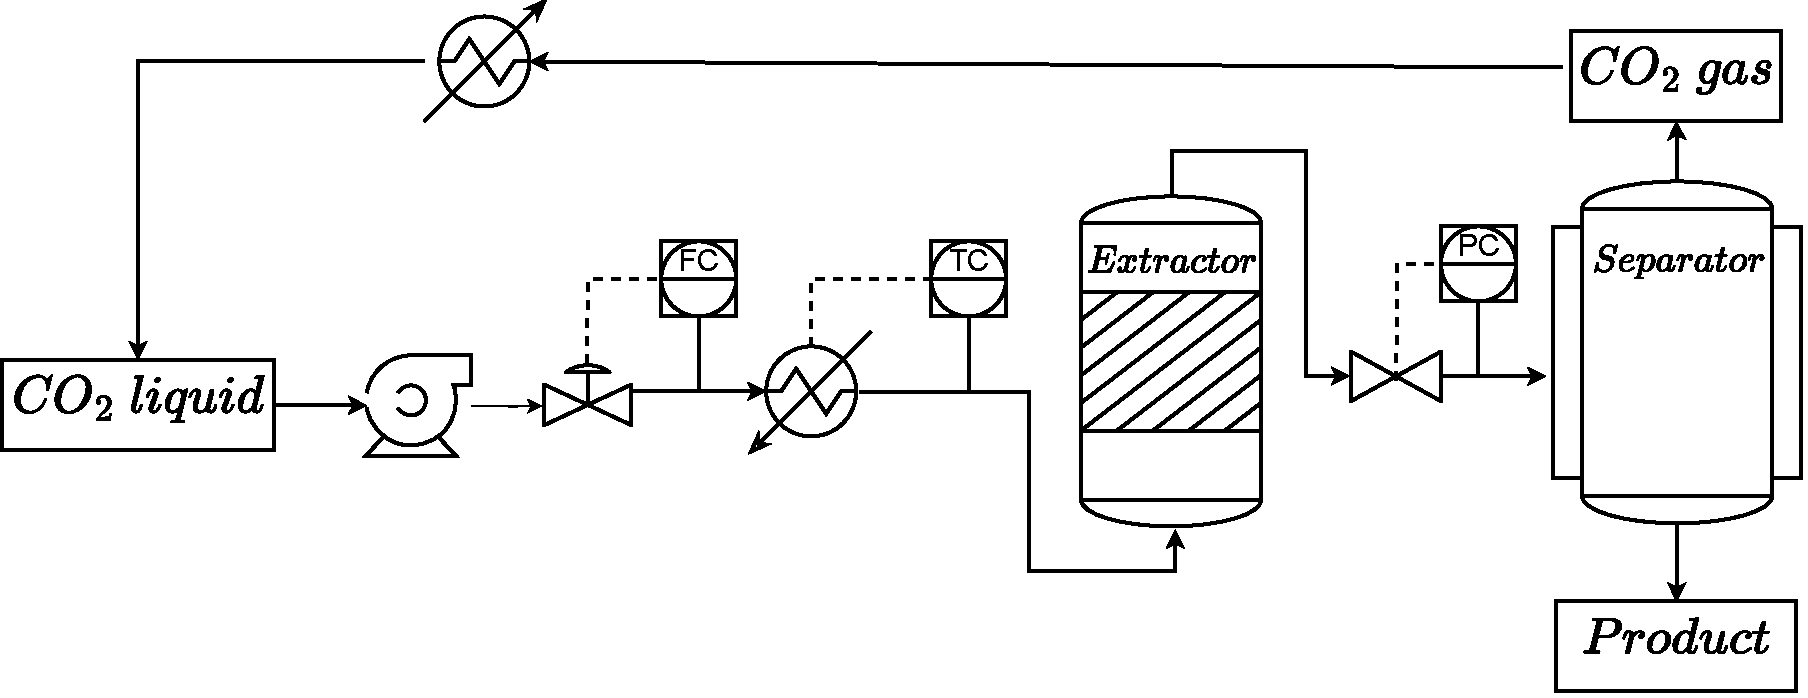
\includegraphics[width=\columnwidth]{Figures/PFD.drawio.pdf}
	\caption{Process flow diagram.}
	\label{fig: SFE_drawing}
\end{figure}

%\subfile{Sections/Literature_Review}
Design of experiments (DoE) is a structured approach that examines how various elements influence a particular result. By evaluating multiple factors at once, DoE allows the uncovering of the impacts of each element and their combinations to be discovered, yielding a comprehensive comprehension of the entire system. DoE begins with the determination of the experiment's objectives and selection of the factors for the study process. DoE aims to obtain the maximum information from an experimental apparatus modelled by devising experiments that will yield the most informative data in a statistical sense for use in parameter estimation and model validation. 

The first conceptualisation of DoE was introduced by \citet{Fisher1935}, who described the fundamental problem of experimental design as deciding which pattern of factor combinations would best reveal the properties of the response that is influenced by the factors. This type of DoE views an experiment as simply connecting inputs with outputs and is therefore called a "black-box experiment design". It aims to select the combinations of factor values that provide the most information on the input-output relationship in the presence of variation. The main class of statistical design techniques of this type of DoE are the so-called factorial methods. These methods are created to measure the additive effects on the response for each input factor and investigate the effects of interactions between factors. Factorial methods are not suitable for situations where constraints exist on the output or internal states. They are better suited for dynamic experiments where inputs and outputs have complex time profiles. However, this group of methods is still widely used due to their simplicity.

\citet{Ramandi2011} conducted a study to identify the variables with the greatest influence on the extraction yield of fatty acids from \textit{Borago officinalis L.} flowers using supercritical fluid extraction (SFE). A full factorial design was employed as the screening method, resulting in a design matrix of 32 runs ($2^5$) carried out randomly to minimise the impact of external factors. The low and high values for the factors were selected based on previous research. After determining the most significant variables, a central composite design was applied to three factors, i.e. temperature, pressure and the volume of the methanol co-solvent, to optimise the SFE conditions. This allowed for the modelling of the response surface by fitting a second-order polynomial.

Similarly, \citet{Caldera2012} conducted a study to optimise the SFE variables, specifically the extraction pressure, extraction temperature and static extraction time, for the maximum extraction of carnosol and carnosic acid from Venezuelan rosemary (\textit{Rosmarinus officinalis L.}) leaves. A $2^3$ full factorial design was initially used to examine these three variables. Based on the statistically significant variables, a Box-Behnken design was employed to create a matrix of 15 experiments, which was used to further optimise the SFE process for maximum carnosol and carnosic acid extraction using response surface methodology.

As opposed to the "black-box" statistical experiment design methods, another form of optimal design has been developed, taking explicit advantage of some knowledge of the structure underlying the system, which is represented by a mathematical model, particularly in the form of differential and algebraic equations. The model-based experiment design approach is characterised by the following:

\begin{enumerate}
	\item explicit use of model equations and current parameters to predict the "information content" of the subsequent experiment
	\item application of an optimisation framework for solving the resulting numerical problem
\end{enumerate}

After an initial data set has been collected and fitted to a mathematical model, the model undergoes further analysis. Additional experiments may be needed to differentiate between competing models that pass the preliminary tests. Once inadequate models have been rejected, the remaining model may undergo another round of experiment design to enhance the precision of its parameters. This paper focuses on the final step of the validation procedure, known as model-based design of experiments (m-DoE), aimed at improving parameter precision. To the best of the authors' knowledge, m-DoE has not been applied to any case of supercritical extraction, so the following literature review provides examples of applications in crystallisation and pharmacology processes.

\citet{Chung2000} applied model-based experimental design to a batch crystallisation process with a cooling jacket. A dynamic programming formulation minimises the volume of the confidence hyper-ellipsoid for the estimated nucleation and growth parameters over the supersaturation profile and the seed characteristics, namely, crystal mass, mean size and width of seed distribution. As a result, the accuracy of the parameter estimates can be improved by identifying the optimal temperature profile.

\citet{Duarte2019} investigated compartment models incorporating Michaelis-Menten elimination kinetics for pharmacological applications. The authors designed both static and dynamic experiments for 2- and 3-compartment models using D-optimality criteria. The dynamic experiments for both models involved the determination of the initial concentration in the first compartment and the optimisation of the mass flow rate profile of the drug entering this compartment.

This study is, to the authors knowledge, the first application of m-DoE with a D-optimality criterion to SFE, contrasted with prior SFE studies that relied on static factorial/RSM designs. Calculations are performed on the full dynamic model to compute exact trajectory-wise Jacobians that drive both the sensitivity study and the information measure. On the experimental-design side, the traditional approach of D-criterion formulate a practically implementable DoE with piecewise-constant inputs and a quadratic move-penalty. The m-DoE is solved for various values of pressure (which is assumed to be cosntant during each batch) to assess the non-trivial impact of operating conditions on the model output.

% ===================================================
% Section: Main
% ===================================================

%\subfile{Sections/Model}
\section{Materials and methods} \label{CH: Materials and methods}

\subsection{Governing equations} \label{CH:Governing_equations_chapter}
The governing equations for a quasi-one-dimensional flow were derived by following the work of \citet{Anderson1995}. A quasi-one-dimensional flow refers to a fluid flow scenario which assumes that the flow properties are uniformly distributed across any cross-section. This simplification is typically applied when the cross-sectional area of the flow channel changes, such as through irregular shapes or partial filling of an extractor. According to this assumption, velocity and other flow properties change solely in the flow direction.

As discussed by \citet{Anderson2023}, all flows are compressible, but some can be treated as incompressible since the velocities are low. This assumption leads to the incompressible condition: $\nabla \cdot u =0$, which is valid for constant density (strictly incompressible) or varying density flow. The assumption allows for removal of acoustic waves and large perturbations in density and/or temperature. In the 1-D case, the incompressibility condition becomes $\frac{du}{dz} = 0$, so the fluid velocity is constant along $z-$ direction.

The set of quasi-one-dimensional governing equations in Cartesian coordinates is described by Equations \ref{EQ: CompressibleEuler_1} - \ref{EQ: CompressibleEuler_3}:

{\footnotesize
	\begin{align}
		\label{EQ: CompressibleEuler_1}
		\cfrac{\partial \left( \rho_f A_f \right) }{\partial t} + \cfrac{\partial \left( \rho_f A_f v \right)}{\partial z} &= 0 \\
		\cfrac{\partial \left( \rho_f v A_f \right) }{\partial t} + \cfrac{\partial \left( \rho_f A_f v^2 \right)}{\partial z} &= -A_f \cfrac{\partial P}{\partial z} \label{EQ: CompressibleEuler_2} \\
		\cfrac{\partial \left( \rho_f e A_f \right) }{\partial t} + \cfrac{\partial \left( \rho_f A_f v e\right)}{\partial z} &= -P\cfrac{\left( A_f v \right)}{\partial z} + \cfrac{\partial}{\partial z} \left( k \cfrac{\partial T}{\partial z} \right)   
		\label{EQ: CompressibleEuler_3}
	\end{align}  
}

where $\rho_f$ is the fluid density, $A_f$ is the function which describes a change in the cross-section, $v$ is the velocity, $P$ is the total pressure, $e$ is the internal energy of the fluid, $T$ is the temperature, $t$ is time, and $z$ is the spatial direction.

Equation \ref{EQ: CompressibleEuler_1}-\ref{EQ: CompressibleEuler_3} are the quasi-one-dimensional conservation laws for a variable-area duct representing a packed bed under the quasi-1D and low-Mach assumptions. Equation (\ref{EQ: CompressibleEuler_1}) (continuity) enforces conservation of mass is convected axially with velocity. Equation (\ref{EQ: CompressibleEuler_2}) (axial momentum) balances the momentum of the fluid parcel with the pressure gradient. The viscous wall/porous drag and body forces are neglected in the control-oriented model because pressure is imposed and nearly uniform in the low-velocity regime. Equation (\ref{EQ: CompressibleEuler_3}) (energy) transports internal energy by advection, includes pressure work, and accounts for axial heat conduction via the effective conductivity. The details on treatment of the governing equations are presented in Section \ref{CH: Extraction_model}.

\subsection{Extraction model} \label{CH: Extraction_model}
\subsubsection{Continuity equation} \label{CH: Continuity}

The previously derived quasi-one-dimensional continuity equation (Equation \ref{EQ: CompressibleEuler_1}) is redefined by incorporating the function $A_f = A\phi$. This modification differentiates constant and varying terms, where the varying term accounts for changes in the cross-sectional area available for the fluid. Equation \ref{EQ: Continuity_differential} shows the modified continuity equation:

{\footnotesize
	\begin{equation} \label{EQ: Continuity_differential}
		\frac{\partial (\rho_f \phi)}{\partial t} + \frac{\partial (\rho_f v A\phi)}{\partial z} = 0
	\end{equation}
}
where $A$ is the total cross-section of the extractor and $\phi$ describes the porosity along the extractor.

Assuming that the porosity and mass flow rate are constant in time, the temporal derivative becomes the mass flux F, and the spatial derivative can be integrated along $z$ as

{\footnotesize
	\begin{equation}
		\int \frac{\partial (\rho_f v A \phi )}{\partial z} dz = F \rightarrow F=\rho_f v A\phi
	\end{equation}
}

To simplify the system dynamics, it is assumed that $F$ is a control variable and affects the whole system instantaneously (due to $\nabla \cdot u = 0$), which allows the velocity profile that satisfies mass continuity based on $F$, $\phi$ and $\rho_f$ to be found:

{\footnotesize
	\begin{equation} \label{EQ:Velocity_1}
		v = \cfrac{F}{\rho_f A\phi} 
	\end{equation}
}

Similarly, superficial velocity may be introduced:

{\footnotesize
	\begin{equation} \label{EQ:Velocity_2}
		u = v \phi = \cfrac{F}{\rho_f A }
	\end{equation}
}

The fluid density $\rho_f$ can be obtained from the Peng-Robinson equation of state if the temperature and thermodynamic pressure are known along $z$. Variation in fluid density may occur due to pressure or inlet temperature changes. In a non-isothermal case, in Equations \ref{EQ:Velocity_1} and \ref{EQ:Velocity_2} $\rho_f$ is considered to be the average fluid density along the extraction column.

\subsubsection{Mass balance for the fluid phase} \label{CH: Mass_balance_fluid}

Equation \ref{Model_fluid} describes the movement of the solute in the system, which is constrained to the axial direction due to the quasi-one-dimensional assumption. Given that the solute concentration in the solvent is negligible, the fluid phase is described as pseudo-homogeneous, with properties identical to those of the solvent itself. It is also assumed that the thermodynamic pressure remains constant throughout the device. The analysis further simplifies the flow dynamics by disregarding the boundary layer near the extractor's inner wall. This leads to a uniform velocity profile across any cross-section perpendicular to the axial direction. Thus, the mass balance equation includes convection, diffusion and kinetic terms representing the fluid phase behaviour:

{\footnotesize
	\begin{equation}
		\label{Model_fluid}
		\frac{\partial c_f}{\partial t}
		+ \frac{1}{\phi} \frac{\partial \left( c_f u\right)}{\partial z}
		= \frac{1-\phi}{\phi} r_e
		+ \frac{1}{\phi} \frac{\partial}{\partial z} \left( D^M_e \frac{\partial c_f}{\partial z} \right)
	\end{equation}
}

where $c_f$ represents the solute concentration in the fluid phase, $r_e$ is the mass transfer kinetic term and $D^M_e$ is the axial dispersion coefficient.

\subsubsection{Mass balance for the solid phase} \label{Mass_balance_solid}

As given by Equation \ref{Model_solid}, the solid phase is considered to be stationary, without convection and diffusion terms in the mass balance equation. Therefore, the only significant term in this equation is the kinetic term of Equation \ref{Model_kinetic_basic}, which connects the solid and fluid phases. For simplicity, the extract is represented by a single pseudo-component: 

{\footnotesize
	\begin{equation} 
		\label{Model_solid}
		%		{\scriptsize\begin{equation}
				\cfrac{\partial c_s}{\partial t} = \underbrace{ -  r_e }_{\text{Kinetics}}
		\end{equation} }
		
		\subsubsection{Kinetic term} \label{CH: Kinetic}
		
		As the solvent flows through the fixed bed, CO$_2$ molecules diffuse into the pores, adsorb on the inner surface and form a film due to solvent-solid matrix interactions. The dissolved solute diffuses from the particle's core through the solid-fluid interface, the pore and the film into the bulk. Figure \ref{fig: SFE_Mechanism} shows the mass transfer mechanism, where the mean solute concentration in the solid phase is denoted as $c_s$, and the equilibrium concentrations at the solid-fluid interface are denoted as $c_s^*$ and $c_p^*$ for the solid and fluid phases, respectively. The concentration of the solutes in the fluid phase in the centre of the pore is denoted as $c_p$. As the solute diffuses through the pore, its concentration changes, reaching $c_{pf}$ at the opening. Then, the solute diffuses through the film around the particle and reaches bulk concentration $c_f$. The two-film theory describes the solid-fluid interface inside the pore. The overall mass transfer coefficient can be determined from the relationship between the solute concentration in one phase and its equilibrium concentration.
		
		\begin{figure}[h!]
			\centering
			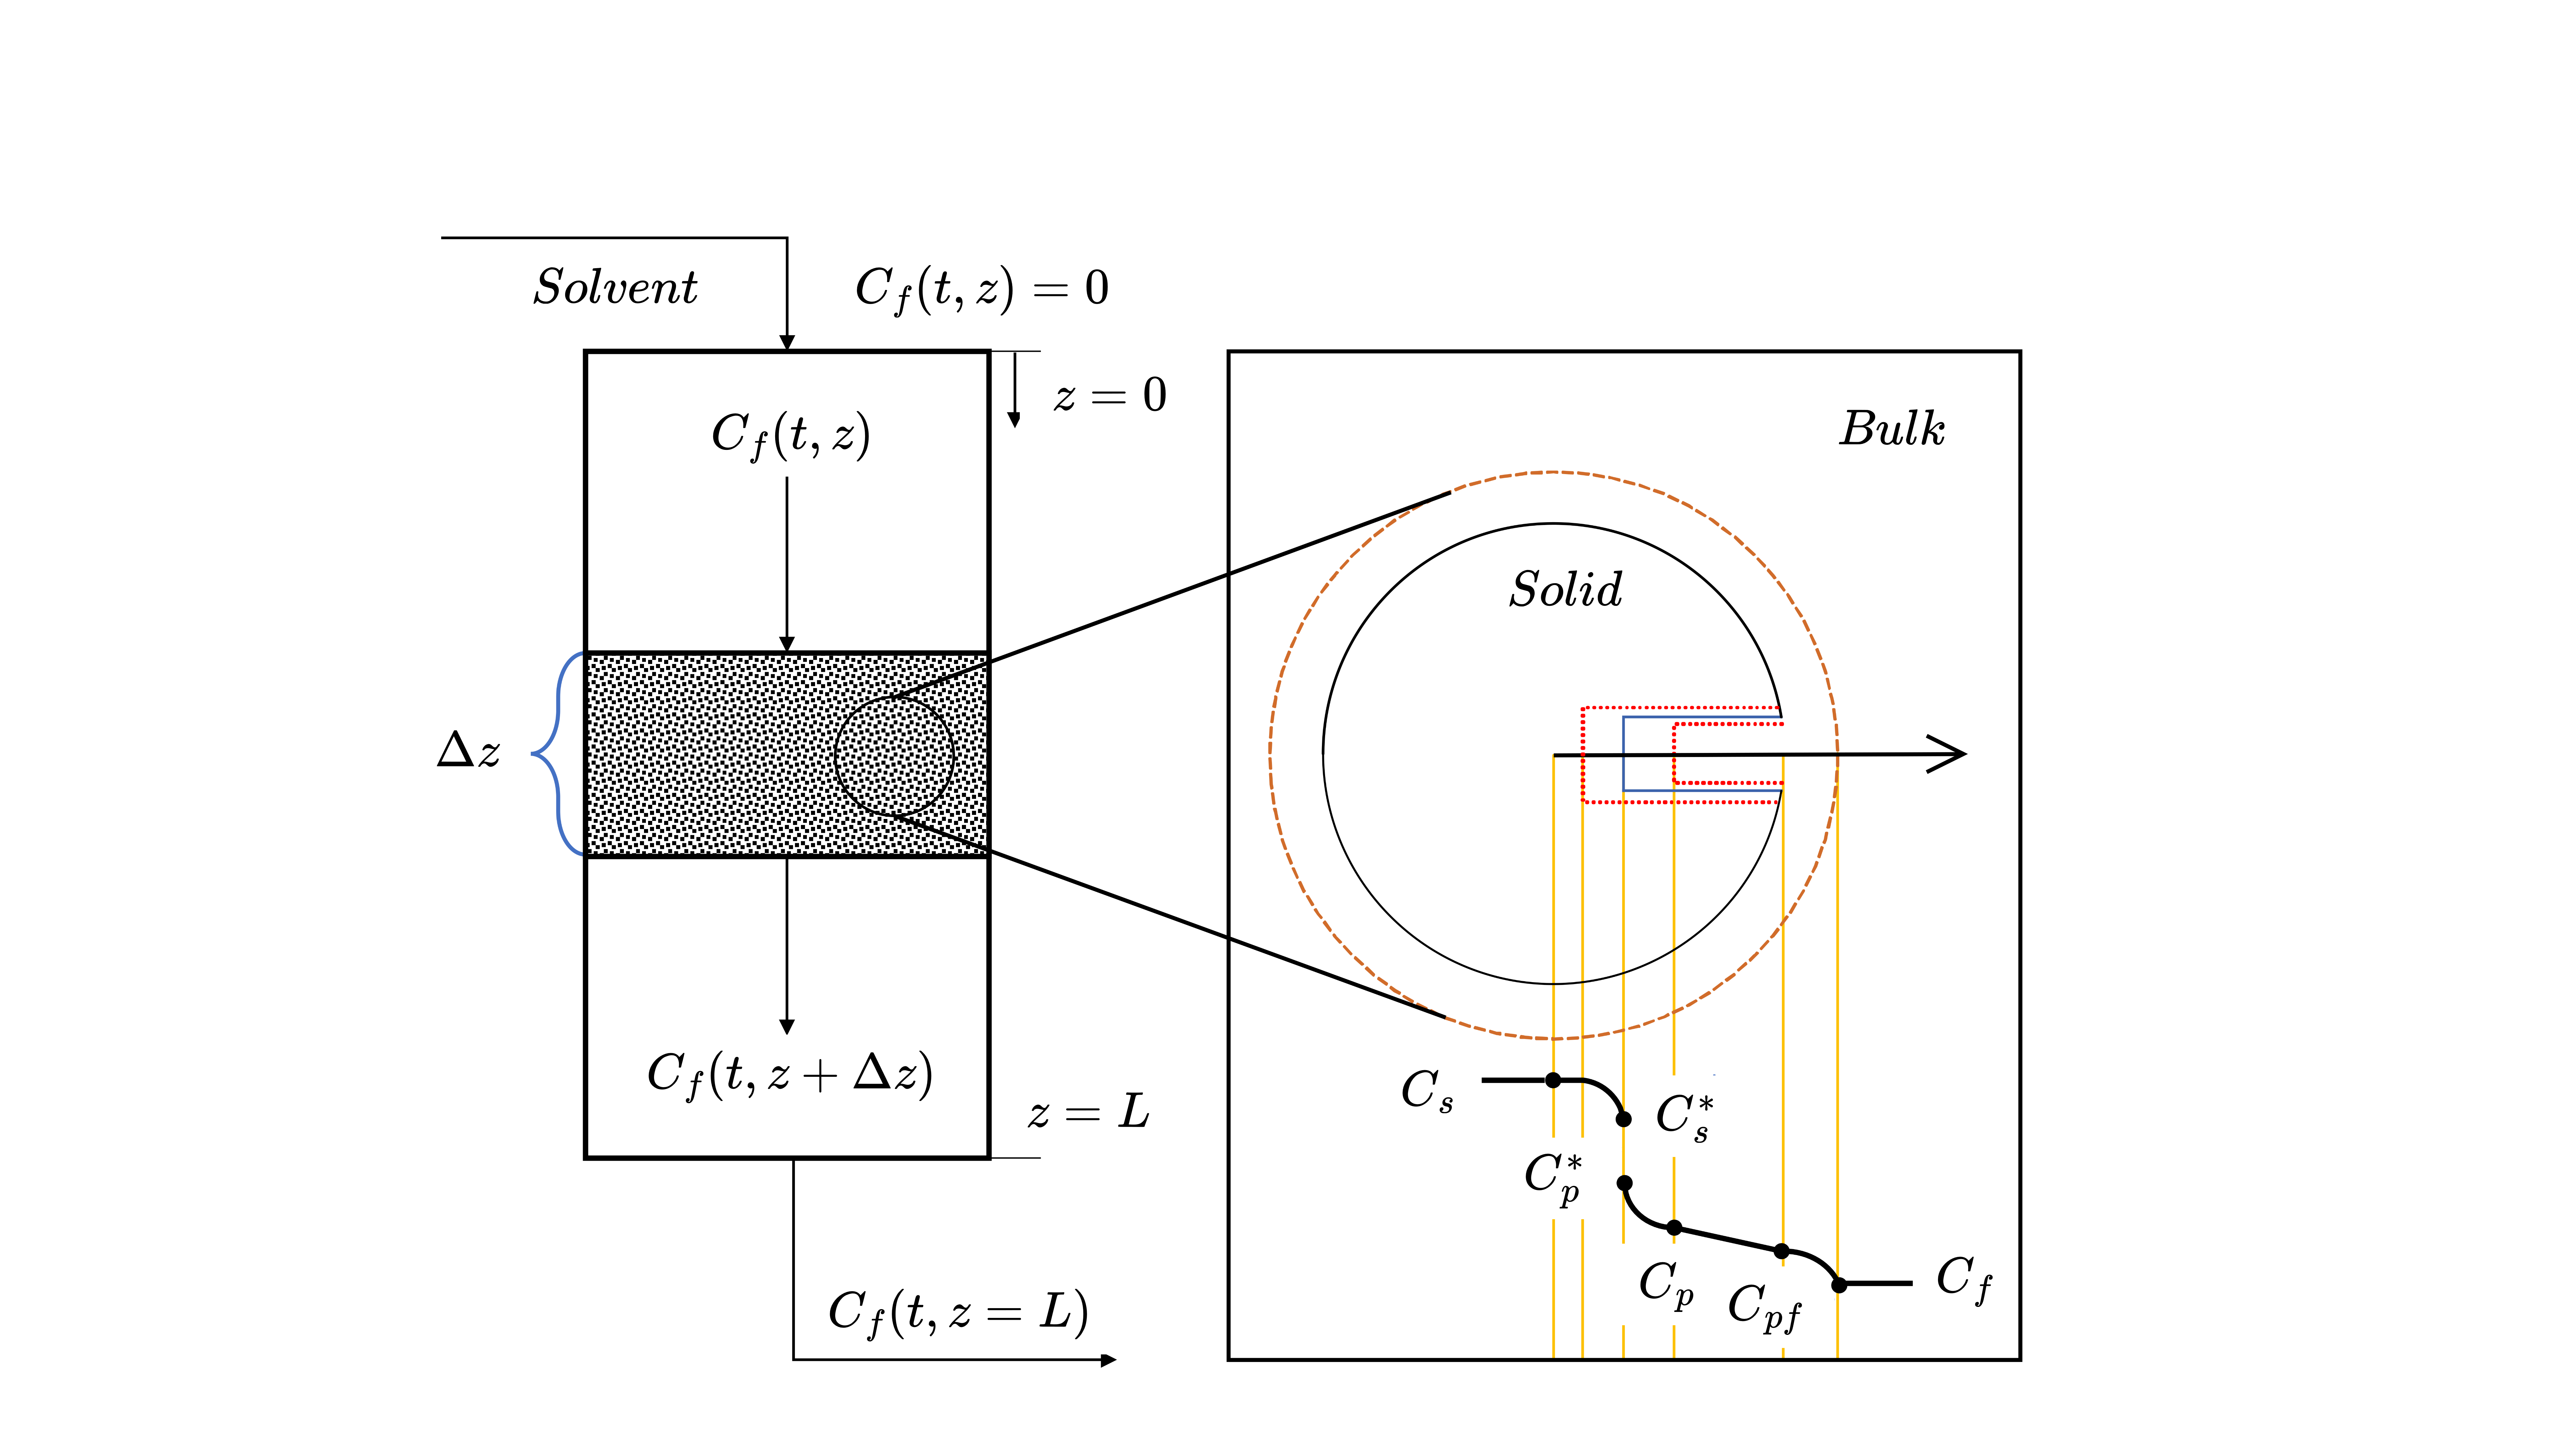
\includegraphics[trim = 45cm 0cm 60cm 20cm,clip,width=0.85\columnwidth]{Figures/SFE_PFD.drawio.png}	
			\caption{Mass transfer mechanism.}
			\label{fig: SFE_Mechanism}
		\end{figure}
		
		\citet{Bulley1984} suggest a process where the driving force for extraction is given by the difference between the concentration of the solute in the bulk, $c_f$, and in the centre of the pore, $c_p^*$. According to the equilibrium relationship, the concentration $c_p^*$ is in equilibrium with $c_s$. The rate of extraction is thus $r_e\left(c_f - c^*_p(c_s)\right)$. In contrast, \citet{Reverchon1996} proposes a driving force given by the difference between $c_s$ and $c_p^*$. As given by Equation \ref{Model_kinetic_basic}, the concentration $c_p^*$ is determined by the equilibrium relationship with $c_f$:
		
		{\footnotesize
			\begin{equation} \label{Model_kinetic_basic}
				r_e = \cfrac{D_i}{\mu l^2 }\left(c_s - c_p^* \right)
		\end{equation} }
		
		where $\mu$ is sphericity, $l$ a characteristic dimension of particles that can be defined as $l = r/3$, $r$ is the mean particle radius, $D_i$ corresponds to the overall diffusion coefficient and $c_P^*$ is the concentration at the solid-fluid interface (which according to the internal resistance model is supposed to be at equilibrium with the fluid phase). 
		
		According to \citet{Bulley1984}, a linear equilibrium relationship (Equation \ref{Linear_equilibirum}) can be used to find the equilibrium concentration of the solute in the fluid phase $c_f^*$ based on the concentration of the solute in the solid phase $c_s$:
		
		{\footnotesize
			\begin{align} \label{Linear_equilibirum}
				c_f^* &= k_p c_s
		\end{align} }
		
		The volumetric partition coefficient $k_p$ acts as an equilibrium constant between the solute concentration in one phase and the corresponding equilibrium concentration at the solid-fluid interphase. \citet{Spiro2007} proposed a definition of the mass partition coefficient $k_m$ and the solid density $\rho_s$ as 
		
		{\footnotesize
			\begin{align}
				k_m = \cfrac{k_p \rho_s}{\rho_f}
		\end{align} }
		
		According to \citet{Reverchon1996}, the kinetic term becomes
		
		{\footnotesize
			\begin{equation}
				\label{Model_kinetic_no_sat}
				r_e = \cfrac{D_i}{ \mu l^2 } \left(c_s - \cfrac{\rho_s c_f}{k_m \rho_f} \right)
		\end{equation} }
		
		%\subfile{Saturation}
		\subsubsection{Uneven solute distribution in the solid phase} \label{CH: Gamma_Function}
		
		Following the idea of the broken-and-intact cell (BIC) model (\citet{Sovova2017}), the internal diffusion coefficient $D_i$ is considered to be a product of the reference value of $D_i^R$ and the exponential decay function $\gamma$, as given by Equation \ref{EQ: C_sat_function}:
		
		{\footnotesize
			\begin{equation}
				D_i = D_i^R \gamma(c_s) = D_i^R \exp \left( - \Upsilon \left( 1-\cfrac{ c_s }{c_{s0}} \right) \right) \label{EQ: C_sat_function}
		\end{equation} }
		
		where  ${\color{black}\Upsilon}$ describes the curvature of the decay function. Equation \ref{Model_kinetic} describes the final form of the kinetic term:
		
		{\footnotesize
			\begin{equation}
				\label{Model_kinetic}
				r_e = \cfrac{D_i^R \gamma }{ \mu l^2 } \left( c_s  - \cfrac{\rho_s c_f }{ k_m \rho_f }  \right)
		\end{equation} }
		
		The $\gamma$ function limits the solute's availability in the solid phase. Similarly to the BIC model, the solute is assumed to be contained inside the cells, some of which are open because the cell walls have been broken by grinding, with the rest remaining intact. The diffusion of solute from a particle's core takes more time than the diffusion of solute close to the outer surface. The same idea can be represented by the decaying internal diffusion coefficient, where the decreasing term is a function of the solute concentration in the solid. 
		
		An alternative interpretation of the decay function $\gamma$ involves taking into account the porous structure of the solid particles, where the pores are initially saturated with the solute. During extraction, the solute within these pores gradually dissolves into the surrounding fluid. Initially, the solute molecules near the pore openings dissolve and diffuse rapidly due to the short diffusion paths. As extraction progresses, the dissolution front moves deeper into the pore structure and solute from the inner regions of the pores begins to dissolve. The diffusion of solute molecules from the interior of the pores to the external fluid becomes progressively slower because the effective diffusion path length increases. This lengthening of the diffusion path enhances mass transfer resistance, reducing the overall diffusion rate. 
		
		In an extreme case, this model could be compared with the shrinking core (SC) model presented by \citet{Goto1996}, where the particle radius is reduced as the solute content in the solid phase decreases. In the SC model, the reduction in particle size leads to significant changes in both the diffusion path length and the surface area available for mass transfer. The diminishing particle size increases the diffusion path within the remaining solid core and decreases the external surface area, both of which contribute to a slower extraction rate. When comparing this to the varying diffusion coefficient in our model, some conceptual similarities can be noticed.
		
		\subsubsection{Empirical correlations}
		
		The empirical correlations for $D_i$ and $\Upsilon$ were derived by \citet{Sliczniuk2024} and validated for temperatures of $30 - 40~^\circ C$, pressures of $100 - 200$ bar and mass flow rates of $3.33-6.67 \cdot 10^{-5}$ kg/s. Figures \ref{fig:Correlation_Di} and \ref{fig:Correlation_Gamma} show the results of multiple linear regression applied to parameter estimation solutions and selected independent variables. The region marked with the white dashed line represents the confidence region where the model has been tested. Both correlations should be equal or greater than zero to avoid unphysical behaviour such as reverse mass transfer. The multiple linear regression functions are combined with the rectifier function to ensure non-negativity.
		
		\begin{figure}[!ht]
			\centering
			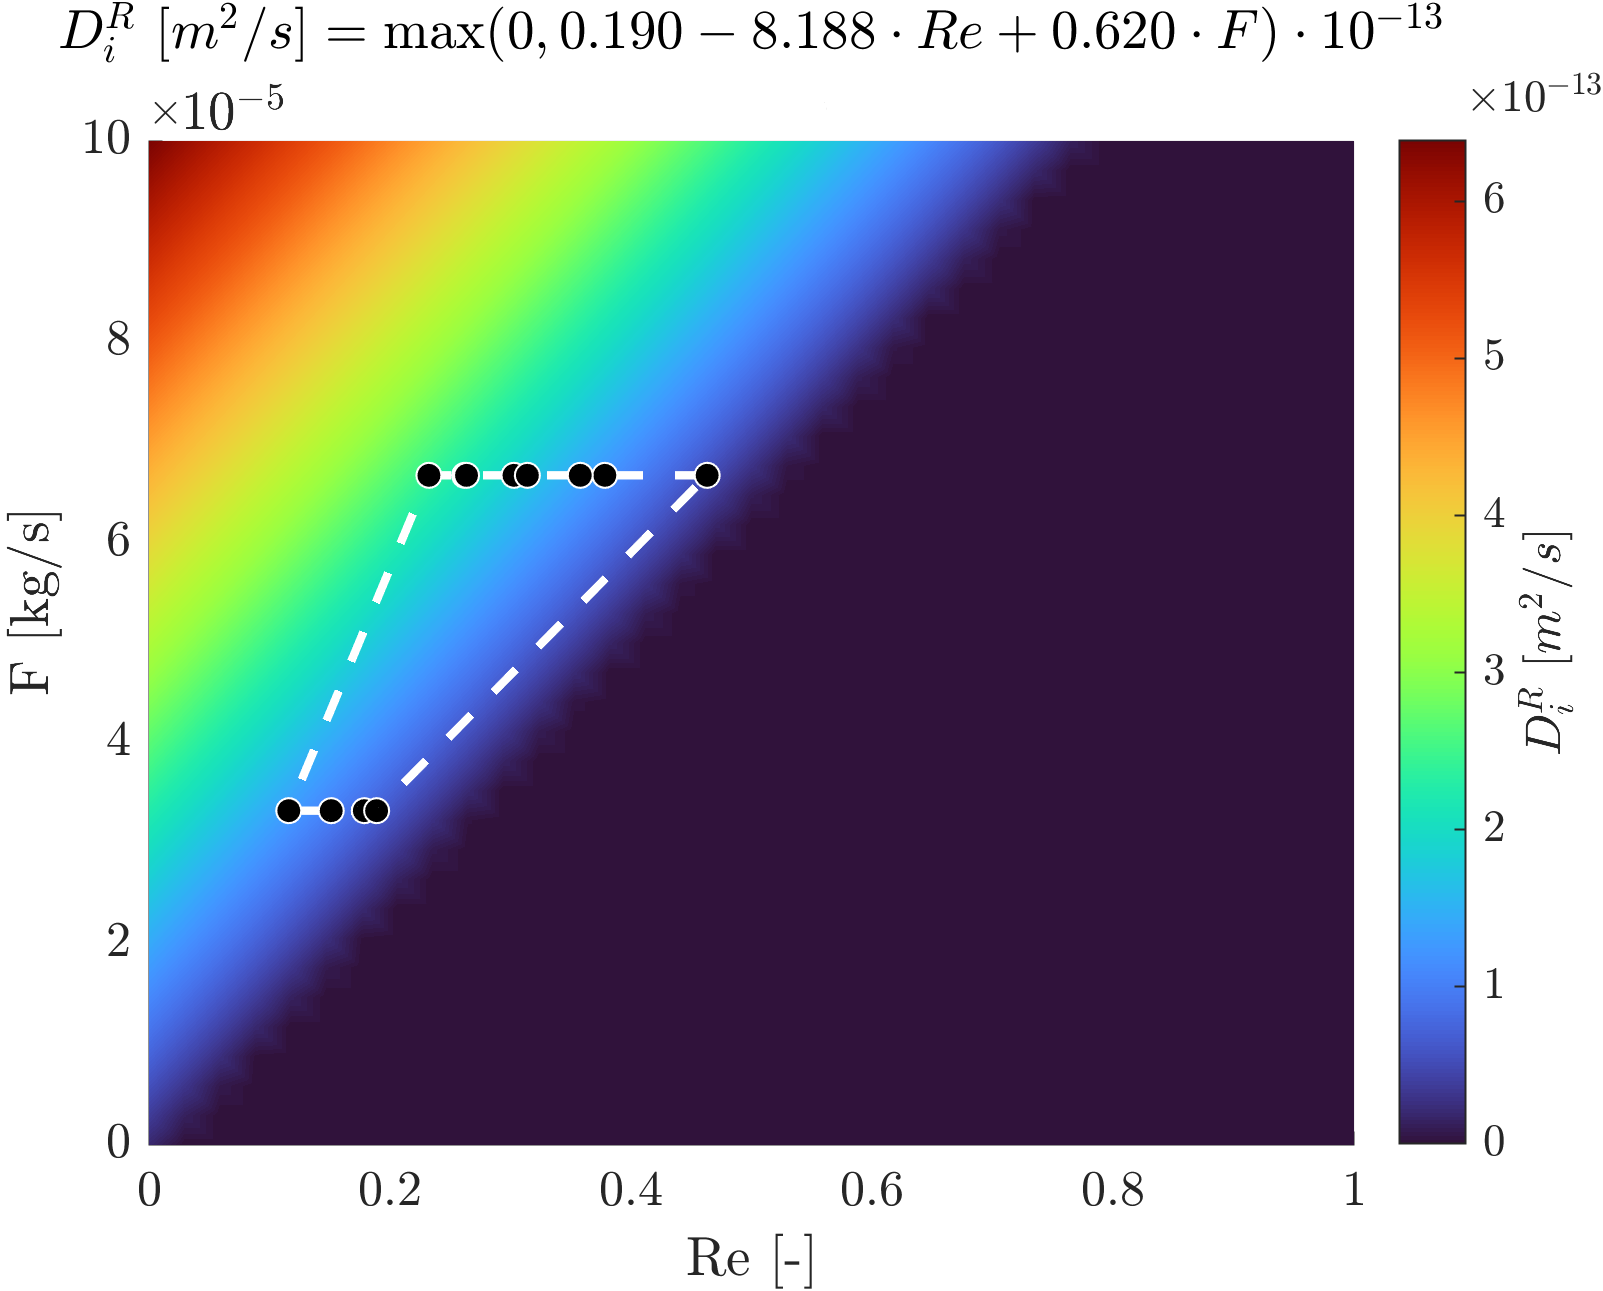
\includegraphics[trim = 0.0cm 0.0cm 0.0cm 0.0cm,clip,width=0.9\columnwidth]{/Di_1.png}
			\caption{Multiple linear regression $D_i^R = f(Re, F)$.}
			\label{fig:Correlation_Di}
		\end{figure}
		
		\begin{figure}[!ht]
			\centering
			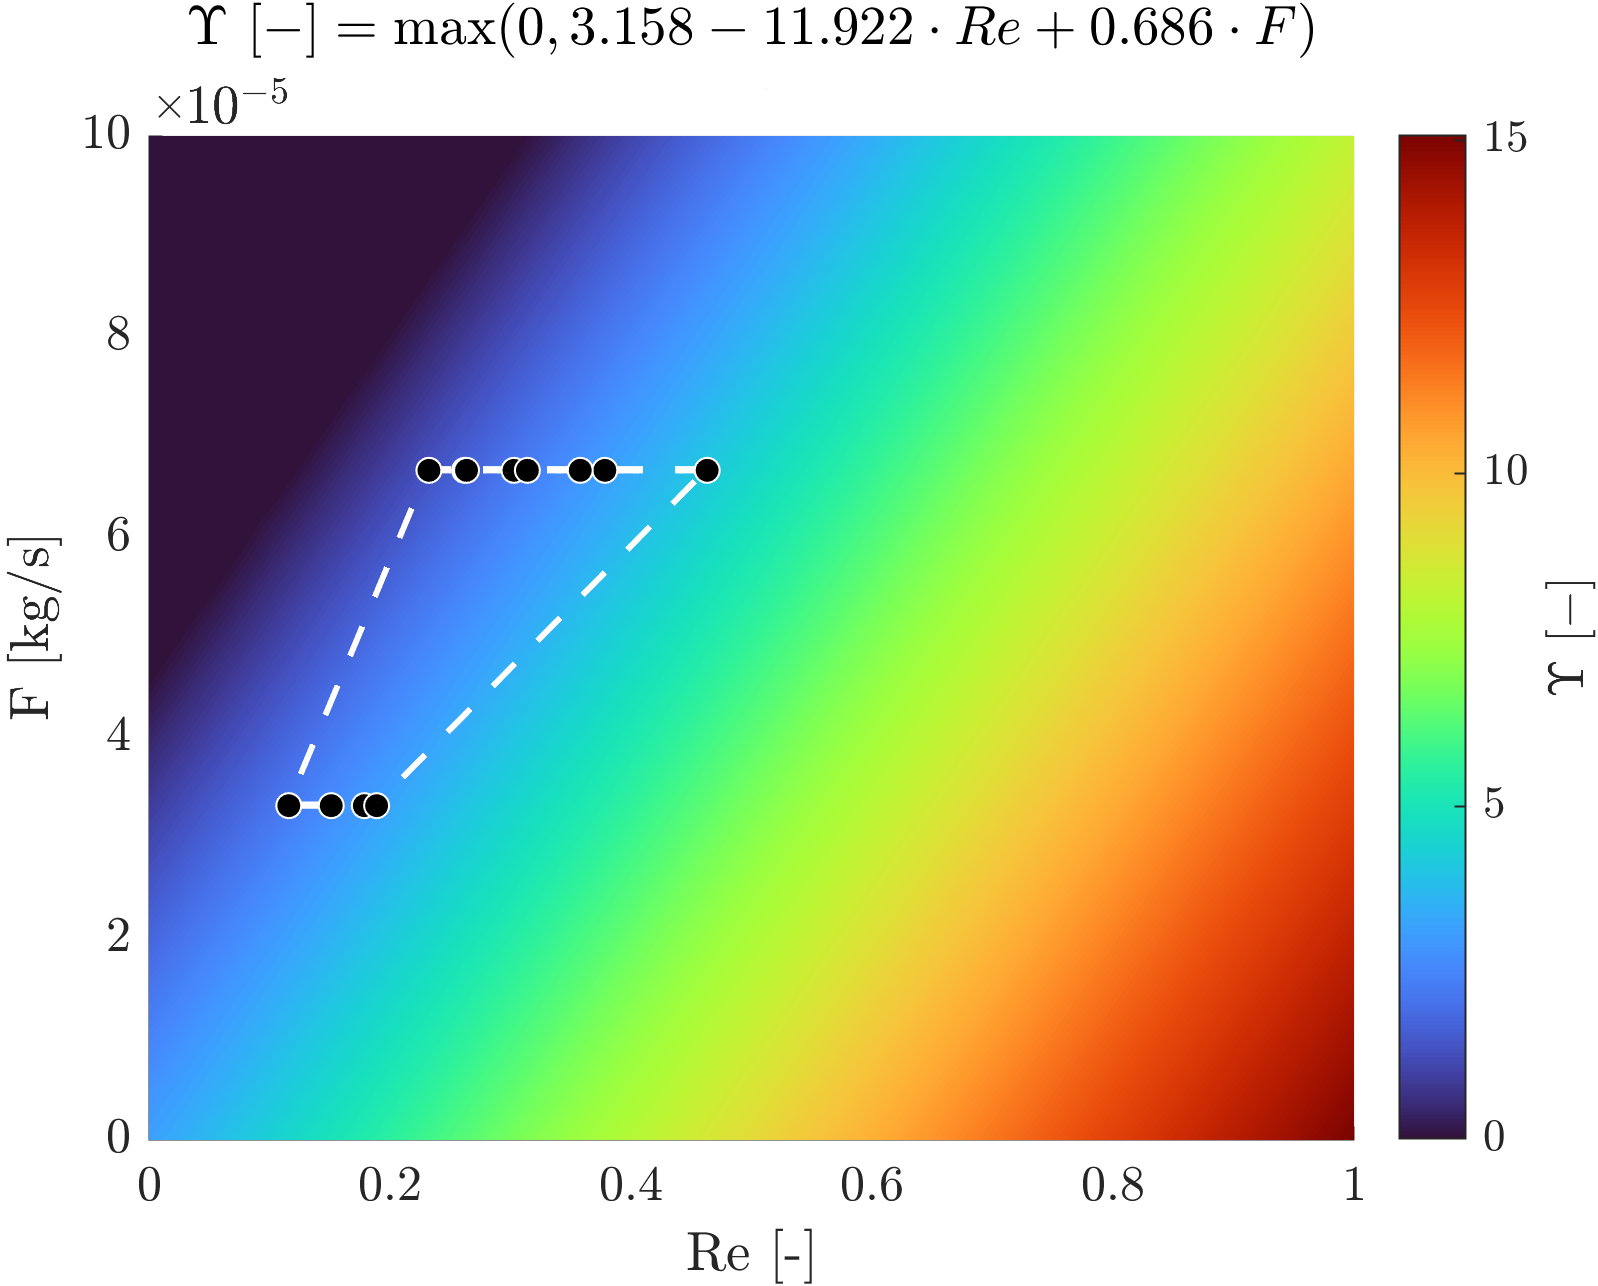
\includegraphics[trim = 0.0cm 0.0cm 0.0cm 0.0cm,clip,width=0.9\columnwidth]{/Gamma_1.png}
			\caption{Multiple linear regression $\Upsilon = f(Re, F)$.}
			\label{fig:Correlation_Gamma}
		\end{figure}
		
		The residuals between predicted and observed values were used to compute an unbiased estimate of the error variance. This variance, combined with the inverse of the design matrix's Gram matrix, yielded the covariance matrix of the coefficient estimates. The standard deviations (standard errors) of the coefficients were then obtained as the square roots of the diagonal elements of this covariance matrix. The variance-covariance is presented in Table \ref{tab:Uncertainty}.
		
		\begin{table}[h!]
			\centering
			\resizebox{0.75\columnwidth}{!}{%
				$
				\begin{gathered}
					\begin{array}{c|ccc}
						& \sigma(D_i^R(0)) & \sigma(Re) & \sigma(F) \\
						\hline
						\sigma(D_i^R(0)) & 0.0817  &  0.0065 &  -0.0139 \\
						\sigma(Re)       & 0.0065  &  1.6908 &  -0.0825 \\
						\sigma(F)        & -0.0139 & -0.0825 &  0.0065 \\
					\end{array}
					\\[1.5em]
					\begin{array}{c|ccc}
						& \sigma(\Upsilon(0)) & \sigma(Re) & \sigma(F) \\
						\hline
						\sigma(\Upsilon(0)) & 0.1727  &  0.0138 &  -0.0294 \\
						\sigma(Re)          & 0.0138  &  3.5732 &  -0.1744 \\
						\sigma(F)           & -0.0294 & -0.1744 &  0.0137 \\
					\end{array}
				\end{gathered}
				$
			}
			\caption{Variance–covariance matrices for $D_i^R$ (top) and $\Upsilon$ (bottom)}
			\label{tab:Uncertainty}
		\end{table}
				
		\subsubsection{Heat balance} \label{CH: heat_balance}
		
		The heat balance equation describes the evolution of enthalpy in the system, given by Equation \ref{EQ:Enthalpy_equation}:
		
		{\footnotesize
			\begin{equation} \label{EQ:Enthalpy_equation}
				\cfrac{\partial \left(\rho_f {\color{black}h} A_f\right)}{\partial t} = - \cfrac{\partial \left( \rho_f {\color{black}h}  v \right)}{\partial z} + \cfrac{\partial \left(P A_f\right)}{\partial t} + \cfrac{\partial}{\partial z} \left( k \cfrac{\partial T}{\partial z} \right)
			\end{equation}
		}
		
		If the value of enthalpy $h$ is known from the time evolution of the energy equation and pressure $P$ is known from measurement, then the temperature $T$ can be reconstructed based on the departure function. The departure function is a mathematical function that characterises the deviation of a thermodynamic property (enthalpy, entropy or internal energy) of a real substance from that of an ideal gas at the same temperature and pressure. As presented by \citet{Gmehling2019}, the enthalpy departure function for the Peng-Robinson equation of state is defined by Equation \ref{EQ:Enthalpy_PR}:
		
		{\scriptsize
			\begin{equation}
				{\color{black}h}-{\color{black}h}^{id}={\color{black}R}T \left[{\color{black}T_r}({\color{black}Z}-1) -2.078(1+{\color{black}\kappa} ){\sqrt { {\color{black}\alpha}\left(T\right) } } \ln \left(\cfrac{{\color{black}Z}+\left( 1+\sqrt{2} \right){\color{black}B}}{{\color{black}Z}+\left( 1-\sqrt{2} \right){\color{black}B}}\right)\right]
				\label{EQ:Enthalpy_PR}
			\end{equation}				
		}
		
		where $\alpha$ is defined as $\left( 1+\kappa \left( 1 - \sqrt{T_r} \right) \right)^2$, $T_r$ is the reduced temperature, $P_r$ is the reduced pressure, $Z$ is the compressibility factor, $\kappa$ is a quadratic function of the acentric factor and $B$ is calculated as $0.07780\frac{P_r}{T_r}$.
		
		Equation \ref{EQ:Enthalpy_PR} requires a reference state, which is assumed to be $T_{ref}=298.15$ K and $P_{ref}=1.01325$ bar.
		
		A root finder can be used to find a temperature value that minimises the difference between the value of enthalpy coming from the heat balance and the departure functions. The root-finding procedure is repeated at every time step to find a temperature profile along the spatial direction $z$.
		
		{\footnotesize
			\begin{equation}
				\min_T \left( \underbrace{h\left(t,x\right)}_{\text{Heat balance}} - \underbrace{h\left(T,P,\rho_f\left(T,P\right)\right)}_{\text{Departure function}} \right)^2
				\label{EQ:Enthalpy_root}
			\end{equation}
		}
		
		\subsubsection{Pressure term} \label{CH: Pressure}
		
		As explained in Section \ref{CH:Governing_equations_chapter}, the pressure in the low-velocity region remains nearly constant due to the small pressure wave propagation occurring at the speed of sound. Under such conditions, the term $\partial P/\partial t$ can be approximated by a forward difference equation, describing the pressure change over a small time step $\Delta t$. The pressure $P$ in the system is treated as a state variable, while the incoming pressure at the new time step $P_{in}$ is treated as a control:
		
		{\footnotesize
			\begin{equation}
				\frac{\partial {\color{black}P}}{\partial t} \approx \frac{{\color{black}P_{in}} - {\color{black}P} }{\Delta t}
		\end{equation}}
		
		Such a simplified equation allows for instantaneous pressure. In a real system, the pressure dynamics would depend on the behaviour of the pump and the back-pressure regulator, which introduce additional inertia and resistance to pressure changes, leading to gradual pressure build-up.
		
		\subsubsection{Extraction yield} \label{CH: Yield}
		
		The process yield is calculated according to Equation \ref{Model_measurment_1}, as presented by \citet{Sovova1994a}. The measurement equation evaluates the solute's mass at the extraction unit outlet and sums it up. The integral form of the measurement (Equation \ref{Model_measurment_1}) can be transformed into the differential form (Equation \ref{Model_measurment_2}) and augmented with the process model.
		
		{\footnotesize
			\begin{align} 
				\label{Model_measurment_1}
				y &= \int_{t_0}^{t_f} \cfrac{F}{\rho_f} c_f \biggr\rvert_{z=L} dt \\
				\cfrac{dy}{dt} &= \qquad \cfrac{F}{\rho_f} c_f \biggr\rvert_{z=L} 
				\label{Model_measurment_2}
		\end{align}	}

		The measurement error can be obtained based on the accuracy of the measuring device, or empirically from the spread of data around the model output. The first approach can be utilised only in the absence of external error sources. Given the imperfections of the experimental setup, such as delayed measurements and residuals of the product in pipes and the draining vessel, it was decided that the second approach is more suitable for this work. Based on the \citet{Sliczniuk2024}, the empirical measurement error was estimated to be 0.03.
		
		\subsubsection{Initial and boundary conditions} 
		It is assumed that the solvent is free of solute at the beginning of the process $c_{f0}=0$, that all the solid particles have the same initial solute content $c_{s0}$ and that the system is isothermal, hence the initial state is $h_0$. The fluid at the inlet is considered not to contain any solute. The initial and boundary conditions are defined as follows:
		
		{\footnotesize
			\begin{align*}
				&c_f(t = 0, z) = 0  && c_s(t = 0, z) = c_{s0} && h(t = 0, z) = h_0 \\
				&c_f(t,   z=0) = 0  && h(t, z=0) = h_{in}  && \frac{\partial c_f(t,z=L)}{\partial x} = 0 \\
				&\frac{\partial h(t,z=L)}{\partial x} = 0   && c_s(t, z=\{0,L\}) = 0 && y(0) = 0 \quad P(0) = P_0 \\
		\end{align*} }
		
		\subsubsection{Discretisation methods}
		
		\begin{figure}[!h]
			\centering
			{\footnotesize
				\begin{align*}
					\dot{x} &= \cfrac{d x}{d t} = 
					\begin{bmatrix}
						\cfrac{d c_{f,1}}{d t} 	  \\
						\vdots					  \\
						\cfrac{d c_{f,N_z}}{d t} \\
						\\ \hline \\
						\cfrac{d c_{s,1}}{d t} 	  \\
						\vdots					  \\
						\cfrac{d c_{s,N_z}}{d t} \\
						\\ \hline \\
						\cfrac{d h_1}{d t} 	  \\
						\vdots 					  \\
						\cfrac{d h_{N_z}}{d t} \\
						\\ \hline \\
						\cfrac{d P}{d t} \\
						\\ \hline \\
						\cfrac{d y}{d t}
					\end{bmatrix}
					=
					\underbrace{\begin{bmatrix}
							G_1 \left( c_f,c_s,h; \Theta \right)\\ 
							\vdots\\ 
							G_{N_z} \left( c_f,c_s,h; \Theta \right)\\ 
							\\ \hline \\ \\
							G_{N_z+1} \left( c_f,c_s,h; \Theta \right)\\ 
							\vdots\\
							G_{2N_z} \left( c_f,c_s,h; \Theta \right)\\ 
							\\ \\ \hline \\ 
							G_{2N_z+1} \left( c_f,c_s,h; \Theta \right) \\
							\vdots\\
							G_{3N_z} \left( c_f,c_s,h; \Theta \right) \\ 
							\\ \\ \hline \\
							G_{3N_z+1} \left( c_f,c_s,h; \Theta \right) \\
							\\ \\ \hline \\
							G_{3N_z+2} \left( c_f,c_s,h; \Theta \right) 
					\end{bmatrix}}_{G \left( x; \Theta \right)} 
			\end{align*} }
			\caption{Discretised state space.}
			\label{fig:discretization}
		\end{figure}
		
		The method of lines is used to transform the process model equations into a set of ODEs denoted by $G(x;\Theta)$. For a derivative to be conservative, it must form a telescoping series. In other words, only the boundary terms should remain after adding all terms coming from the discretisation over a grid, and the artificial interior points should be cancelled out. Discretisation is applied to the conservative form of the model to ensure mass conservation. The backward finite difference is used to approximate the first-order derivative, while the central difference scheme approximates the second-order derivative $z$ direction. The length of the fixed bed is divided into $N_z$, i.e. equally distributed points in the $z$ direction. The state-space model after discretisation is denoted by $x$ and defined as shown in Figure \ref{fig:discretization}, where ${\color{black}x} \in \mathbb{R}^{N_x = 3N_z+2} $ and $\Theta \in \mathbb{R}^{N_\Theta =  N_{\theta} + N_u } $, $N_{\theta}$ is the number of parameters and $N_{u}$ is the number of control variables.
		
		\subsection{Optimal design of experiments} \label{CH: DOE}
		\subsubsection{Bayesian estimation}
		
		After selecting a process model and estimating its parameters based on initial experiments, additional experiments may be planned to further refine the estimates of the model coefficients. An optimal experimental design enables parameters to be estimated without bias and with minimum variance. A model-based approach to experimental design allows for the consideration of system complexity and constraints, such as practical infeasibility due to safety concerns.
		
		Building on the work of \citet{Walter2010} and \citet{Himmelblau1970}, the Bayes theorem can be employed to define a general cost function:
		
		{\footnotesize
			\begin{equation}
				\max p\left(\theta \mid Y, \Xi \right) = \frac{p\left(Y \mid \theta, \Xi\right) p\left(\theta\right)}{\int p\left(Y \mid \theta, \Xi\right) p\left(\theta\right) d\theta} \propto p\left(Y \mid \theta, \Xi\right) p\left(\theta\right)
			\end{equation}
		}
		
		The aim of experimental design is to maximise the posterior probability of estimating $\theta$ ($p\left(\theta \mid Y, \Xi \right)$) given the prior distribution of $\theta$ ($p(\theta)$) obtained from previous experiments, and the likelihood of obtaining observations $Y~\left(p\left(Y \mid \theta, \Xi\right)\right)$ given $\theta$ and experimental conditions $\Xi$. The new observations $Y$, under a set of experimental conditions $\Xi$, are assumed to be normally distributed around the model output $y$, with measurement error covariance $\Sigma_Y$. Similarly, $\theta$ is assumed to be normally distributed around the true parameter values $\hat{\theta}$, with covariance matrix $\Sigma_\theta$ estimated from previous experiments. These probabilities are:
		
		{\footnotesize
			\begin{align} 
				p\left(Y \mid \theta, \Xi \right) &= \frac{|\Sigma_Y|^{-1/2}}{\left(2\pi\right)^{n_Y/2}} \exp\left( -\frac{1}{2} \left(Y - y \right)^\top \Sigma_Y^{-1} \left(Y - y\right) \right) \\
				p\left(\theta\right) &= \frac{|\Sigma_\theta|^{-1/2}}{\left(2\pi\right)^{n_\theta/2}} \exp\left( -\frac{1}{2} \left(\theta - \hat{\theta}\right)^\top \Sigma_\theta^{-1} \left(\theta - \hat{\theta}\right) \right)
			\end{align}
		}
		
		where $n_Y$ is the number of observations and $n_\theta$ is the number of parameters to be estimated. Substituting these expressions into the cost function gives:
		
		{\footnotesize 
			\begin{equation} 
				\ln p\left(\theta \mid Y, \Xi \right) \propto -\frac{1}{2} \left[ \left(Y - y\right)^\top \Sigma_Y^{-1} \left(Y - y\right) + \left(\theta - \hat{\theta}\right)^\top \Sigma_\theta^{-1} \left(\theta - \hat{\theta}\right) \right] 
		\end{equation} }
		
		When linearising the model output around $\hat{\theta}$, the model output becomes $y = y(\hat{\theta}) + J \Delta_\theta$, where $J = \frac{\partial y(\hat{\theta})}{\partial \theta}$ is the Jacobian matrix evaluated at $\hat{\theta}$, and $\Delta_\theta = \theta - \hat{\theta}$. To simplify the equation, the residual term $\Delta_y = Y - y(\hat{\theta})$ is introduced. Substituting these into the expression for $\ln p\left(\theta \mid Y, \Xi \right)$ gives:
		
		{\footnotesize 
			\begin{flalign*} 
				\ln p\left(\theta \mid Y, \Xi \right) &\propto -\frac{1}{2} \left[ \left(\Delta_y - J \Delta_\theta \right)^\top \Sigma_Y^{-1} \left(\Delta_y - J \Delta_\theta \right) + \Delta_\theta^\top \Sigma_\theta^{-1} \Delta_\theta \right] && \\
				&= -\frac{1}{2} \left[ \Delta_y^\top \Sigma_Y^{-1} \Delta_y - 2 \Delta_y^\top \Sigma_Y^{-1} J \Delta_\theta + \Delta_\theta^\top \left( J^\top \Sigma_Y^{-1} J + \Sigma_\theta^{-1} \right) \Delta_\theta \right] &&
		\end{flalign*} }
		
		This equation can be reformulated by expanding the quadratic terms:
		
		{\footnotesize
			\begin{flalign*}
				\ln p\left(Y \mid \theta, \Xi \right) &\propto -\frac{1}{2} \left( \underbrace{r^\top \Sigma_Y^{-1} r}_{\mathcal{C}} - 2 \underbrace{ J^\top \Sigma_Y^{-1} \Delta_y }_{\mathcal{B}} \Delta_\theta + \Delta_\theta^\top \underbrace{\left( J^\top \Sigma_Y^{-1} J + \Sigma_\theta^{-1} \right)}_{\mathcal{A}} \Delta_\theta \right) && \\
				&=-\frac{1}{2} \left( \Delta_\theta^\top \mathcal{A} \Delta_\theta - 2 \mathcal{B}^\top \Delta_\theta + \mathcal{C} \right) &&
			\end{flalign*}
		}
		
		By completing the square, we introduce $\theta^* = \hat{\theta} + \mathcal{A}^{-1} \mathcal{B}$, and the cost function becomes:
		
		{\footnotesize 
			\begin{equation} 
				\ln p\left(\theta \mid Y, \Xi \right) \propto -\frac{1}{2} \left( \left( \theta - \theta^* \right)^\top \mathcal{A} \left( \theta - \theta^* \right) + \mathcal{C} - \mathcal{B}^\top \mathcal{A}^{-1} \mathcal{B} \right) 
		\end{equation} }
		
		It can be observed that the quadratic term represents the spread of the posterior multivariate distribution around the mean $\theta^*$. The constant term $\mathcal{C} - \mathcal{B}^\top \mathcal{A}^{-1} \mathcal{B}$ is independent of $\theta$ and does not affect the shape of the posterior distribution but is still important for normalisation. This constant term is absorbed into the normalising constant of the posterior distribution. It does not affect the estimation of $\theta$ or the shape of the posterior distribution and thus can be neglected when focusing on parameter estimation or experimental design. Therefore, the posterior distribution of $\theta$ given $Y$ and $\Xi$ is:
		
		{\footnotesize \begin{equation} p\left(\theta \mid Y, \Xi \right) \propto \exp \left( -\frac{1}{2} \left( \theta - \theta^* \right)^\top \mathcal{A} \left( \theta - \theta^* \right) \right) \end{equation} }
		
		This is the expression of a multivariate normal distribution with mean $\theta^*$ and covariance matrix $\mathcal{A}^{-1}$:
		
		{\footnotesize \begin{equation} p\left(\theta \mid Y, \Xi \right) = \mathcal{N}\left( \theta^*, \mathcal{A}^{-1} \right) \end{equation} }
		
		As the goal of optimal experimental design is to improve the precision of parameters, the main focus is on the matrix $\mathcal{A}$, which consists of two terms. The first corresponds to the information gained from new observations based on the model and measurement error ($J^\top \Sigma_Y^{-1} J$), while the second is the prior information ($\Sigma_\theta^{-1}$).
		
		\subsubsection{Fisher Information}
		
		The Fisher information $\mathcal{F}$ measures the amount of information that an observable random variable carries about an unknown parameter of the distribution that models the random variable. It is related to the negative expected value of the second derivative of the log-likelihood function with respect to the parameter, providing a measure of how "sensitive" the likelihood is to changes in the parameter value.
		
		{\footnotesize \begin{equation} \mathcal{F}(\theta, \Xi) = -\mathop{\mathbb{E}}_{Y \mid \theta, \Xi} \left[ \frac{\partial^2 \ln p \left( Y \mid \theta, \Xi \right)}{\partial \theta \partial \theta^\top} \right] \end{equation} }
		
		Under regularity conditions, the Fisher information can also be expressed as:
		
		{\footnotesize \begin{equation} \mathcal{F}(\theta, \Xi) = \mathop{\mathbb{E}}_{Y \mid \theta, \Xi} \left[ \left( \frac{\partial \ln p\left( Y \mid \theta, \Xi \right)}{\partial \theta} \right) \left( \frac{\partial \ln p\left( Y \mid \theta, \Xi \right)}{\partial \theta} \right)^\top \right] \end{equation} }
		
		By inserting the expression for $p\left( Y \mid \theta, \Xi \right)$ and performing similar manipulations as in the previous section, the Fisher information becomes:
		
		{\footnotesize \begin{equation} \mathcal{F}(\theta, \Xi) = J^\top \Sigma_Y^{-1} J \end{equation} }
		
		Since the likelihood is Gaussian and linearised, the second derivative of the log-likelihood with respect to $\theta$ simplifies to $J^\top \Sigma_Y^{-1} J$, and its negative expected value yields the same expression because the expectation of the Hessian is constant in this linear approximation.
		
		The Cramer-Rao inequality requires that the covariance of any unbiased estimator $\hat{\theta}$ satisfies:
		
		{\footnotesize \begin{equation} \operatorname{Cov}(\hat{\theta}) \geq \mathcal{F}^{-1}(\theta) \end{equation} }
		
		The precision with which a parameter $\theta$ can be estimated is limited by the Fisher information of the likelihood function. Based on the Cramer-Rao inequality, the Fisher information matrix can be used to calculate the covariance matrices associated with maximum-likelihood estimates.
		
		\subsubsection{Optimal experimental design}
		
		The optimal design of experiments is a statistical concept that refers to the process of planning an experiment that allows parameters to be estimated without bias and with minimum variance. Optimal design ensures that the experiment can provide the most informative data possible. This often involves balancing the study of the main effects and interactions between factors. Moreover, by efficiently planning experiments, optimal design aims to reduce the overall resources required, such as time, materials and manpower.
		
		The methodology for collecting data to estimate the parameters of a specific model is influenced by a series of qualitative decisions made throughout the experimental and modelling process, such as model structure, sensor locations or equipment choices. Once these choices have been made, the experimenter still has some freedom to specify the quantitative experimental conditions (such as temperature, pressure, sampling times, etc.). Experiment design aims to determine the experimental conditions adapted to the final purpose of the modelling.
		
		Considering that each scalar observation in a study can be expressed as $y(\xi_i)$, where the $n_\xi$-dimensional vector $\xi_i$ represents the specific experimental conditions (such as sampling time, operating conditions, etc.) under which the $i$-th observation is gathered. When collecting $n_t$ such observations, the assembly of these $\xi_i$ vectors forms the matrix $\Xi = (\xi_1, \xi_2, \dots, \xi_{n_t})$, which combines all the experimental conditions that need optimisation. To align the design of the experiment with practical realities, it is important to take into account various constraints, such as the total duration of the experiments, the maximum temperature of the inlet stream or the minimum interval between sampling events. The set of all possible combinations for $\Xi$ that adhere to these constraints is denoted as $\bar{\Xi}$.
		
		The formulation of a cost function $j$ allows the framing of optimal experiment design as a constrained optimisation problem. In this context, the optimal experiment, denoted as $\Xi^*$, is:
		
		{\footnotesize \begin{equation} \Xi^* = \arg~\underset{\Xi \in \bar{\Xi}}{\text{opt}}~j\left(\Xi\right) \end{equation} }
		
		The cost function should describe the amount of information obtained from an experiment. For that purpose, it can be assumed that function $\varkappa$ can be related to the covariance matrix $\mathcal{A}^{-1}$ obtained under arbitrary operating conditions:
		
		{\footnotesize \begin{equation} j(\Xi) = \varkappa\left[ \mathcal{A}^{-1}(\theta, \Xi) \right] \end{equation} }
		
		Taking into account that, in the Bayesian estimation framework, the posterior covariance matrix of the parameter estimates is given by $\Sigma = \mathcal{A}^{-1} = \left(J^\top \Sigma_Y^{-1} J + \Sigma_\theta^{-1}\right)^{-1} $. $J$ is the Jacobian matrix of the model outputs with respect to the parameters, $\Sigma_Y$ is the covariance matrix of the measurement errors and $\Sigma_\theta$ is the prior covariance matrix of the parameters.
		
		\begin{figure}[!h]
			\centering
			\resizebox{0.9\columnwidth}{!}{%
				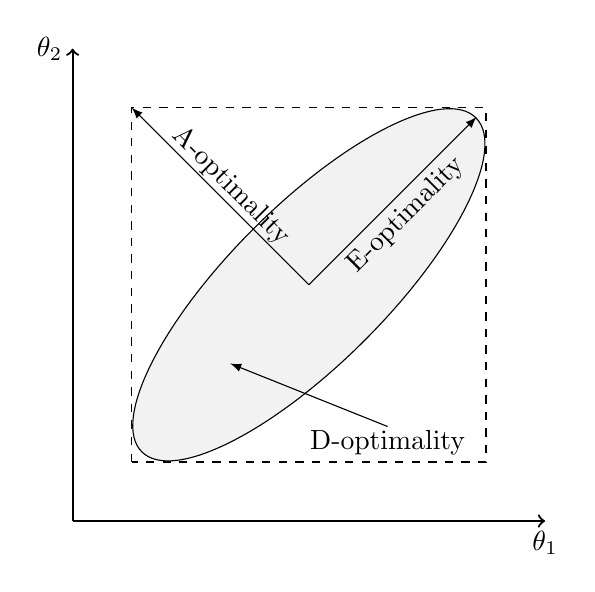
\begin{tikzpicture}
					% Ellipse parameters
					\def\ellipsecenter{(3,3)}
					\def\ellipseA{(0.75,5.25)} % End point for A-optimality arrow
					\def\ellipseB{(5.13,5.13)} % End point for E-optimality arrow
					\def\ellipseC{(4,1.2)}      % End point for D-optimality arrow
					
					% Draw the rotated ellipse
					\draw[fill=gray!10, draw=black, rotate around={45:\ellipsecenter}] \ellipsecenter ellipse (3cm and 1cm);
					
					% Draw the dashed rectangle
					\draw[dashed] (0.75,0.75) rectangle (5.25,5.25);
					
					% Draw the arrows and label them with adjustable positions
					\draw [-latex] \ellipsecenter -- \ellipseA node[yshift=-4cm, xshift=2.5cm,rotate around={-45:\ellipsecenter}] {A-optimality};
					\draw [-latex] \ellipsecenter -- \ellipseB node[yshift=0cm, xshift=-3.9cm,rotate around={45:\ellipsecenter}] {E-optimality};
					\draw [-latex] \ellipseC -- (2,2) node[yshift=-1cm, xshift=2cm] {D-optimality};
					
					% Draw axes
					\draw[thick,->] (0,0) -- (6,0) node[below] {$\theta_1$};
					\draw[thick,->] (0,0) -- (0,6) node[left] {$\theta_2$};
				\end{tikzpicture}
			}%
			\caption{Graphical representation of score functions.}
			\label{fig:score_fun}
		\end{figure}
		
		Equation \ref{EQ:DOE_general} shows the general type of DOE optimality criteria. Some of the DOE criteria have a graphical interpretation, as shown in Figure \ref{fig:score_fun}.
		
		{\footnotesize 
			\begin{align} \label{EQ:DOE_general}
				\varkappa_k\left( \mathcal{A}^{-1}(\theta) \right) &= \left[ \frac{1}{n_\theta} \operatorname{trace}\left( Q \mathcal{A}^{-1}(\theta, \Xi) Q^\top \right)^k \right]^{1/k} & \text{if} \det \mathcal{A}^{-1} \neq 0 \nonumber \\ 
				\varkappa_k\left( \mathcal{A}^{-1}(\theta) \right) &= \infty & \text{if} \det \mathcal{A}^{-1} = 0
		\end{align} }
		
		where $Q$ is the weighting matrix. The special case $k=1$ corresponds to the L-optimality cost function:
		
		{\footnotesize \begin{equation} j_L(\Xi) = \operatorname{trace} \left( Q \mathcal{A}^{-1}(\theta, \Xi) Q^\top \right) \end{equation} }
		
		Selection of $Q = \mathbf{I}_{n\theta}$ corresponds to the A-optimality cost function. An A-optimal experiment minimises the sum of the variances of the parameter estimates (i.e. the trace of the covariance matrix). When $Q$ is diagonal with $[Q]_{ii} = 1/\theta_i$, this corresponds to weighting the parameters inversely by their magnitude, which is associated with relative precision.
		
		Selecting $Q$ as a row vector results in C-optimality, which focuses on linear combinations of parameters. Setting $Q = \mathbf{I}_{n\theta}$ and $k = \infty$ leads to E-optimality, where the design maximises the smallest eigenvalue of the covariance matrix $\mathcal{A}^{-1}(\theta, \Xi)$, thereby minimising the length of the largest axis of the asymptotic confidence ellipsoids.
		
		The most commonly used criterion is D-optimality, which involves $k = 0$ and $Q = \mathbf{I}_{n\theta}$, requiring the minimisation of $\det \mathcal{A}^{-1}(\theta, \Xi)$, or correspondingly, the maximisation of:
		
		{\footnotesize \begin{equation} j_D(\Xi) = \det \mathcal{A}(\theta, \Xi) \end{equation} }
		
		Since $\det A(\theta, \Xi) = 1 / \det \mathcal{A}^{-1}(\theta, \Xi)$, maximising $\det \mathcal{A}$ is equivalent to minimising $\det \mathcal{A}^{-1}$.
		
		The D-optimality (D-OED) criterion originates from the geometric interpretation of the determinant. A two-dimensional matrix with real number entries can represent two linear maps: one mapping the standard basis vectors to the rows and the other to the columns. In both cases, the images of the basis vectors form a parallelogram that represents the image of the unit square under the mapping. The absolute value of the determinant is the area of this parallelogram, reflecting the scale factor by which the matrix transforms areas. The signed value of the determinant indicates the area of the parallelogram, which is negative when the angle from the first to the second defining vector is clockwise. In a multi-dimensional case, the matrix maps the n-cube to an n-dimensional parallelotope. The determinant provides the signed n-dimensional volume of this parallelotope, describing the volume scaling factor of the linear transformation produced by the matrix. Based on this geometrical interpretation, a D-optimal experiment minimises the volume of the asymptotic confidence ellipsoids for the parameters.
		
		\subsubsection{Problem formulation}
		
		Details on the process model can be found in \citet{Sliczniuk2024}. The model's empirical correlations were derived based on laboratory experiments conducted under various but constant operating conditions: $30 - 40~^\circ\text{C}$, $100 - 200$ bar and $3.33 \cdot 10^{-5} - 6.67 \cdot 10^{-5}$ kg/s. This study employs the process model obtained previously to design a set of supplementary experiments with dynamically changing conditions to improve the precision of the correlation for $D_i$. The analysed correlations consist of three independent variables: mass flow rate, pressure and inlet temperature. 
		
		In this work, the decision variables are the inlet temperature ($T^{\text{in}}$) and mass flow rate ($F$), while the pressure is assumed to remain constant during each batch. The optimal design of experiments problem is solved for multiple values of pressure: 100, 125, 150, 175 and 200 bar. The initial state is considered isothermal, so $T^0(z) = T^{\text{in}}(t=0)$.
		
		The decision variables are adjusted every 10 minutes and are kept constant within each interval (piecewise constant controls). These controls have lower and upper bounds that match the validated range of the process model detailed by \citet{Sliczniuk2024}. The sampling time is assumed to be 5 minutes, and the total extraction time 600 minutes.
		
		In a real system, the mass flow rate and inlet temperature cannot be changed instantaneously to any arbitrary value, as they depend on the dynamics of the pump and heat exchanger, respectively. To prevent the bang-bang type of control, a penalty term is introduced. Inspired by control problems such as the linear quadratic regulator, a quadratic penalty term is added to the cost function. This penalty increases the cost function value when there are rapid changes in the decision variables. The matrix $\mathcal{R}$ represents the control cost matrix, with its entries chosen so that the control costs are one order of magnitude lower than $-\ln j_D$. The problem formulation is given by Equation \ref{EQ:Formulation_2}:
		
		{\footnotesize 
			\begin{equation}
				\begin{aligned}
					\Xi^* &= \arg \min_{T^{\text{in}}(t), F(t)} 
					\int_{t_0}^{t_f} \left[ - \ln j_D(\Xi, \dot{x}) + 
					\frac{du(t)^\top}{dt} \, \bar{R} \, \frac{du(t)}{dt} \right] dt, \\
					\text{subject to:} \quad 
					& \dot{x} = G(x, t, \theta; \Xi), \\
					& t_0 = 0 \, \text{min}, \quad t_f = 600 \, \text{min}, \\
					& T^0 = T^{\text{in}}(t=0), \\
					& P(t) \in \{100, 125, 150, 175, 200\} \, \text{bar}, \\
					& 30^\circ\text{C} \leq T^{\text{in}}(t) \leq 40^\circ\text{C}, \\
					& 3.33 \cdot 10^{-5} \leq F(t) \leq 6.67 \cdot 10^{-5}, \\
					& \mathcal{R} = 
					\begin{bmatrix} 
						\mathcal{R}_{FF} & \mathcal{R}_{FT} \\ 
						\mathcal{R}_{TT} & \mathcal{R}_{TF} 
					\end{bmatrix}=
					\begin{bmatrix} 
						0.1 & 0 \\ 
						0 & 0.01 
					\end{bmatrix}, \\
					& \frac{du(t)}{dt} = 
					\begin{bmatrix} 
						\dfrac{dF(t)}{dt} \\ 
						\dfrac{dT^{\text{in}}(t)}{dt} 
					\end{bmatrix}.
				\end{aligned}
				\label{EQ:Formulation_2}
		\end{equation} }
		
		% ===================================================
		% Section: Summary
		% ===================================================
		
		\section{Results}
		To identify a global solution for Equation \ref{EQ:Formulation_2}, the optimisation problem is solved multiple times, each run starting from a random initial solution sampled from a uniform distribution. Figure \ref{fig:scatter} compares the initial and final cost function values across multiple optimisation runs for all pressure cases. The solution with the lowest cost function value is considered the global solution for each case.
		
		\begin{figure}[h!]
			\centering
			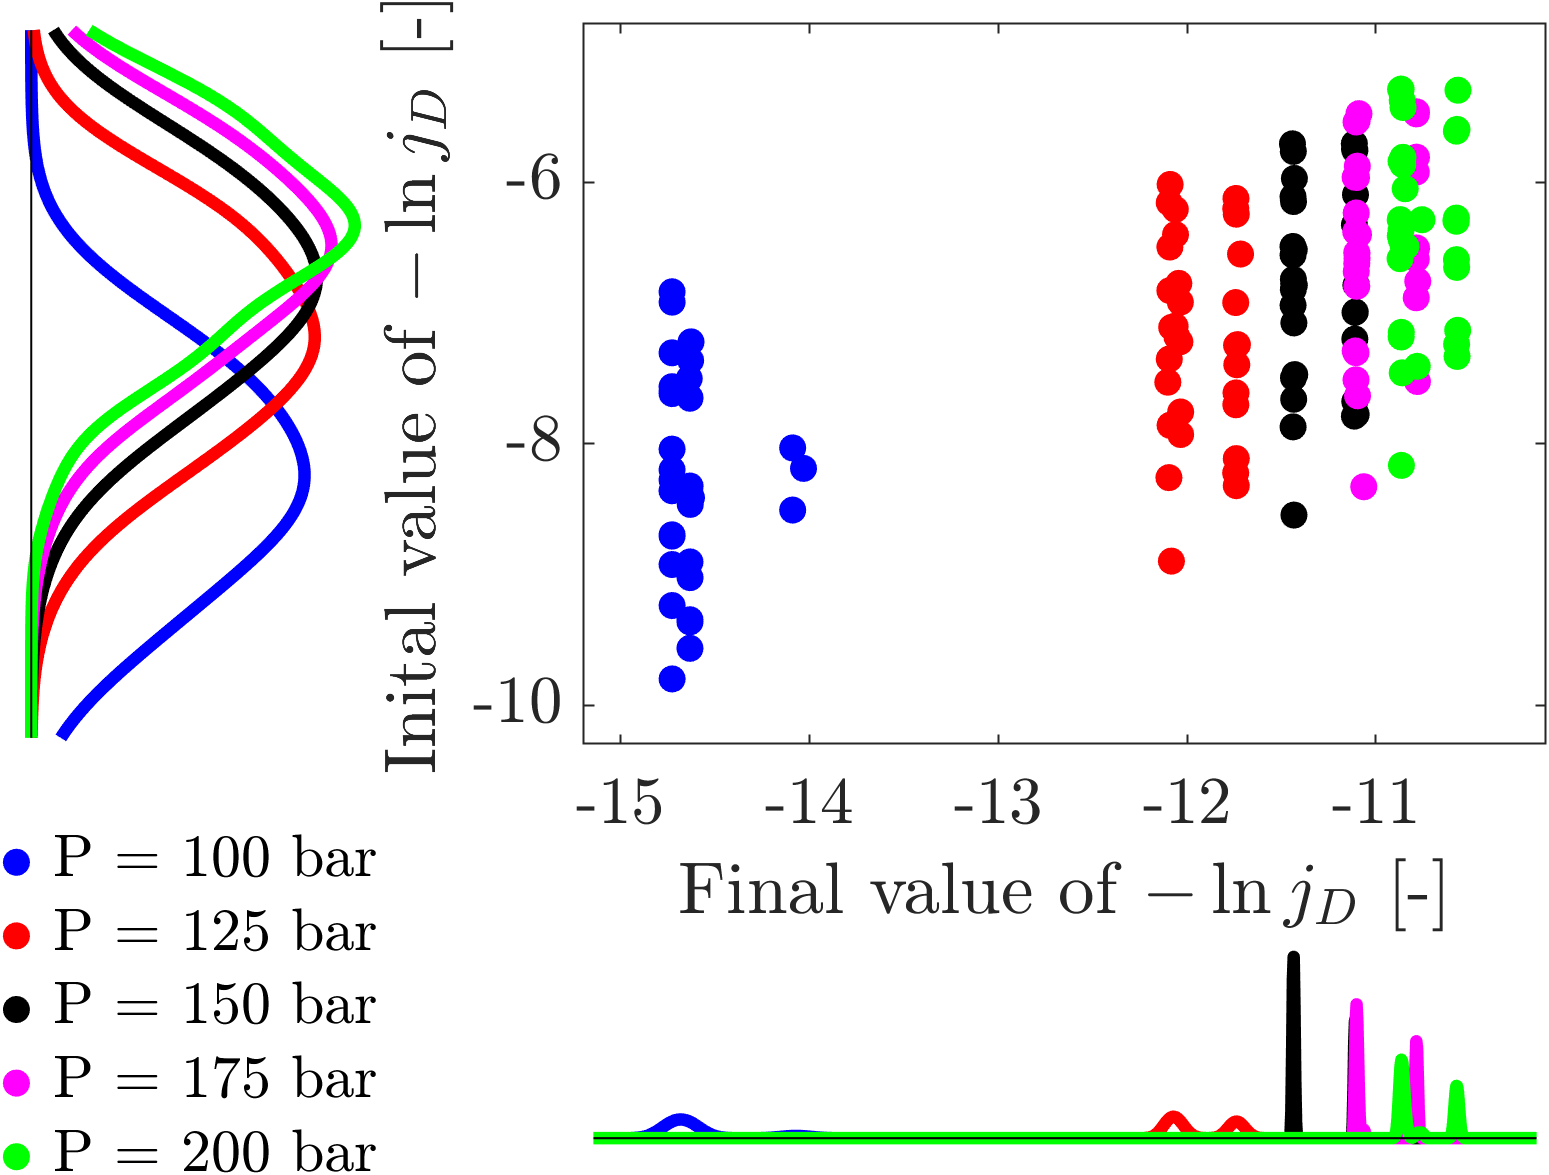
\includegraphics[width=0.90\columnwidth]{Figures/Results/scatter.png}	
			\caption{Initial vs final values of the cost function.}
			\label{fig:scatter}
		\end{figure}
		
		By analysing the locations of the clusters in Figure \ref{fig:scatter}, it can be concluded that experiments conducted near the critical point provide more information regarding the correlation than those conducted farther from it. For each pressure case, the solutions with the lowest value of the objective function are analysed further. The closer the pressure to the critical point, the larger the deviations in the physical properties of $CO_2$ caused by changes in the controls, leading to greater variation in the Reynolds number, and consequently to more informative experiments. 
		
		As presented in Figure \ref{fig:profiles_F}, all mass flow rate profiles initially stay at a minimum value, persisting for 100 to 150 minutes, depending on the pressure. Subsequently, a step-like increase in mass flow rate is observed, with the onset occurring earlier at higher pressures. Between 250 min and 300 min, the mass flow rate stabilises at the value of the upper bound.
		
		\begin{figure}[t!]
			\centering
			\begin{subfigure}[t]{\columnwidth}
				\centering
				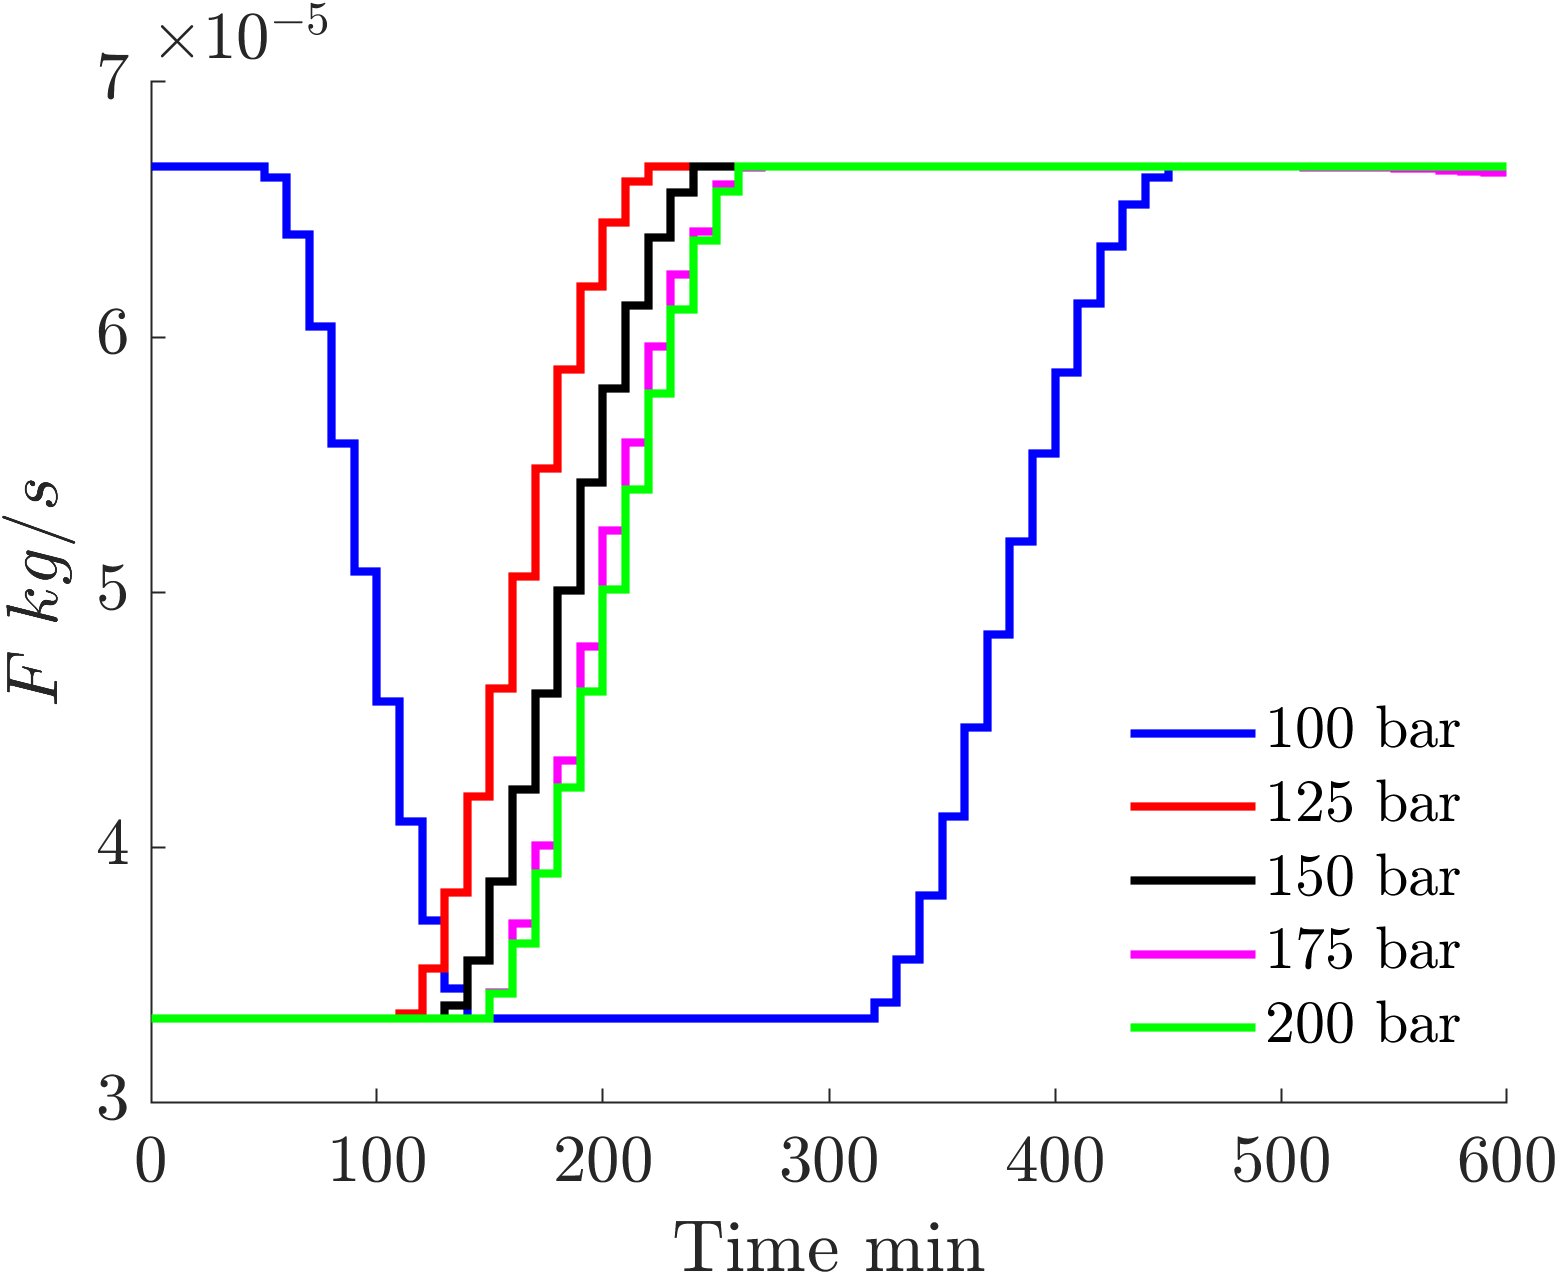
\includegraphics[width=0.90\columnwidth]{Figures/Results/Profile_F.png}	
				\caption{Optimal mass flow rate profiles}
				\label{fig:profiles_F}
			\end{subfigure}%
			\par\bigskip % force a bit of vertical whitespace
			\begin{subfigure}[t]{\columnwidth}
				\centering
				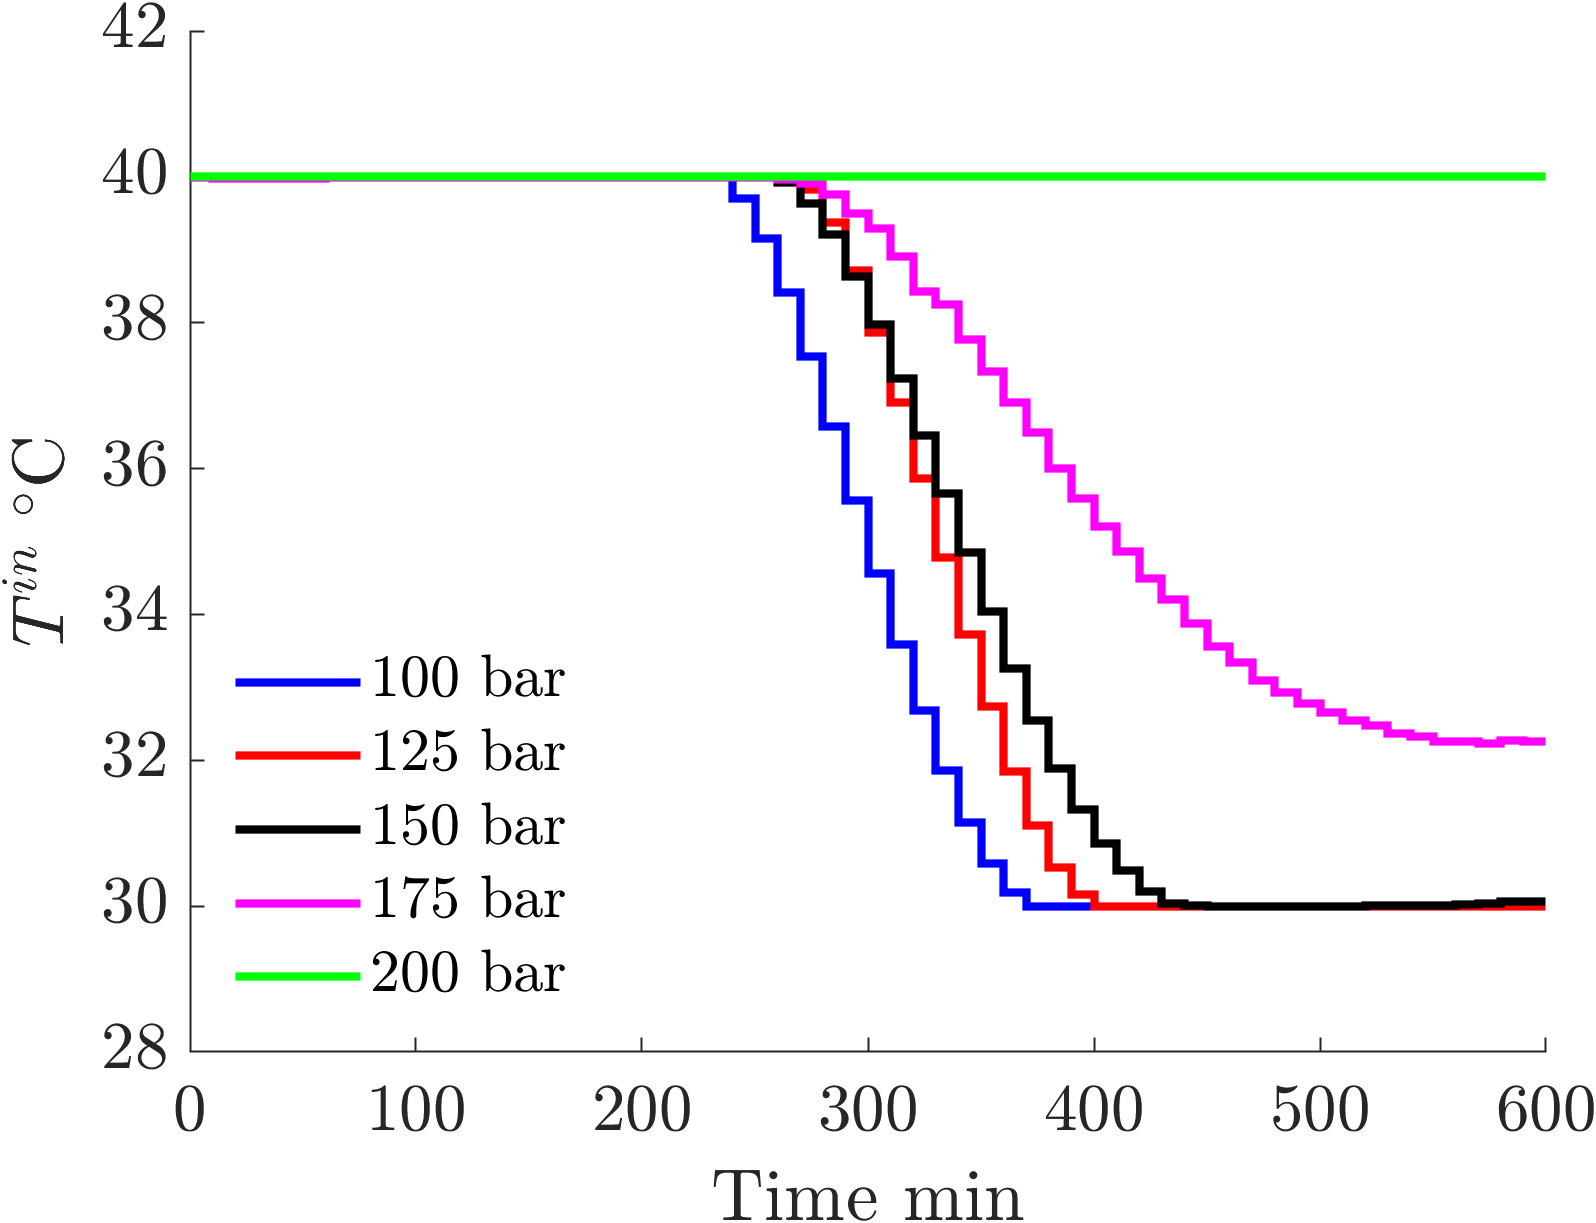
\includegraphics[width=0.90\columnwidth]{Figures/Results/Profile_T.png}	
				\caption{Optimal inlet temperature profile}
				\label{fig:profiles_T}
			\end{subfigure}
			\par\bigskip % force a bit of vertical whitespace
			\begin{subfigure}[t]{\columnwidth}
				\centering
				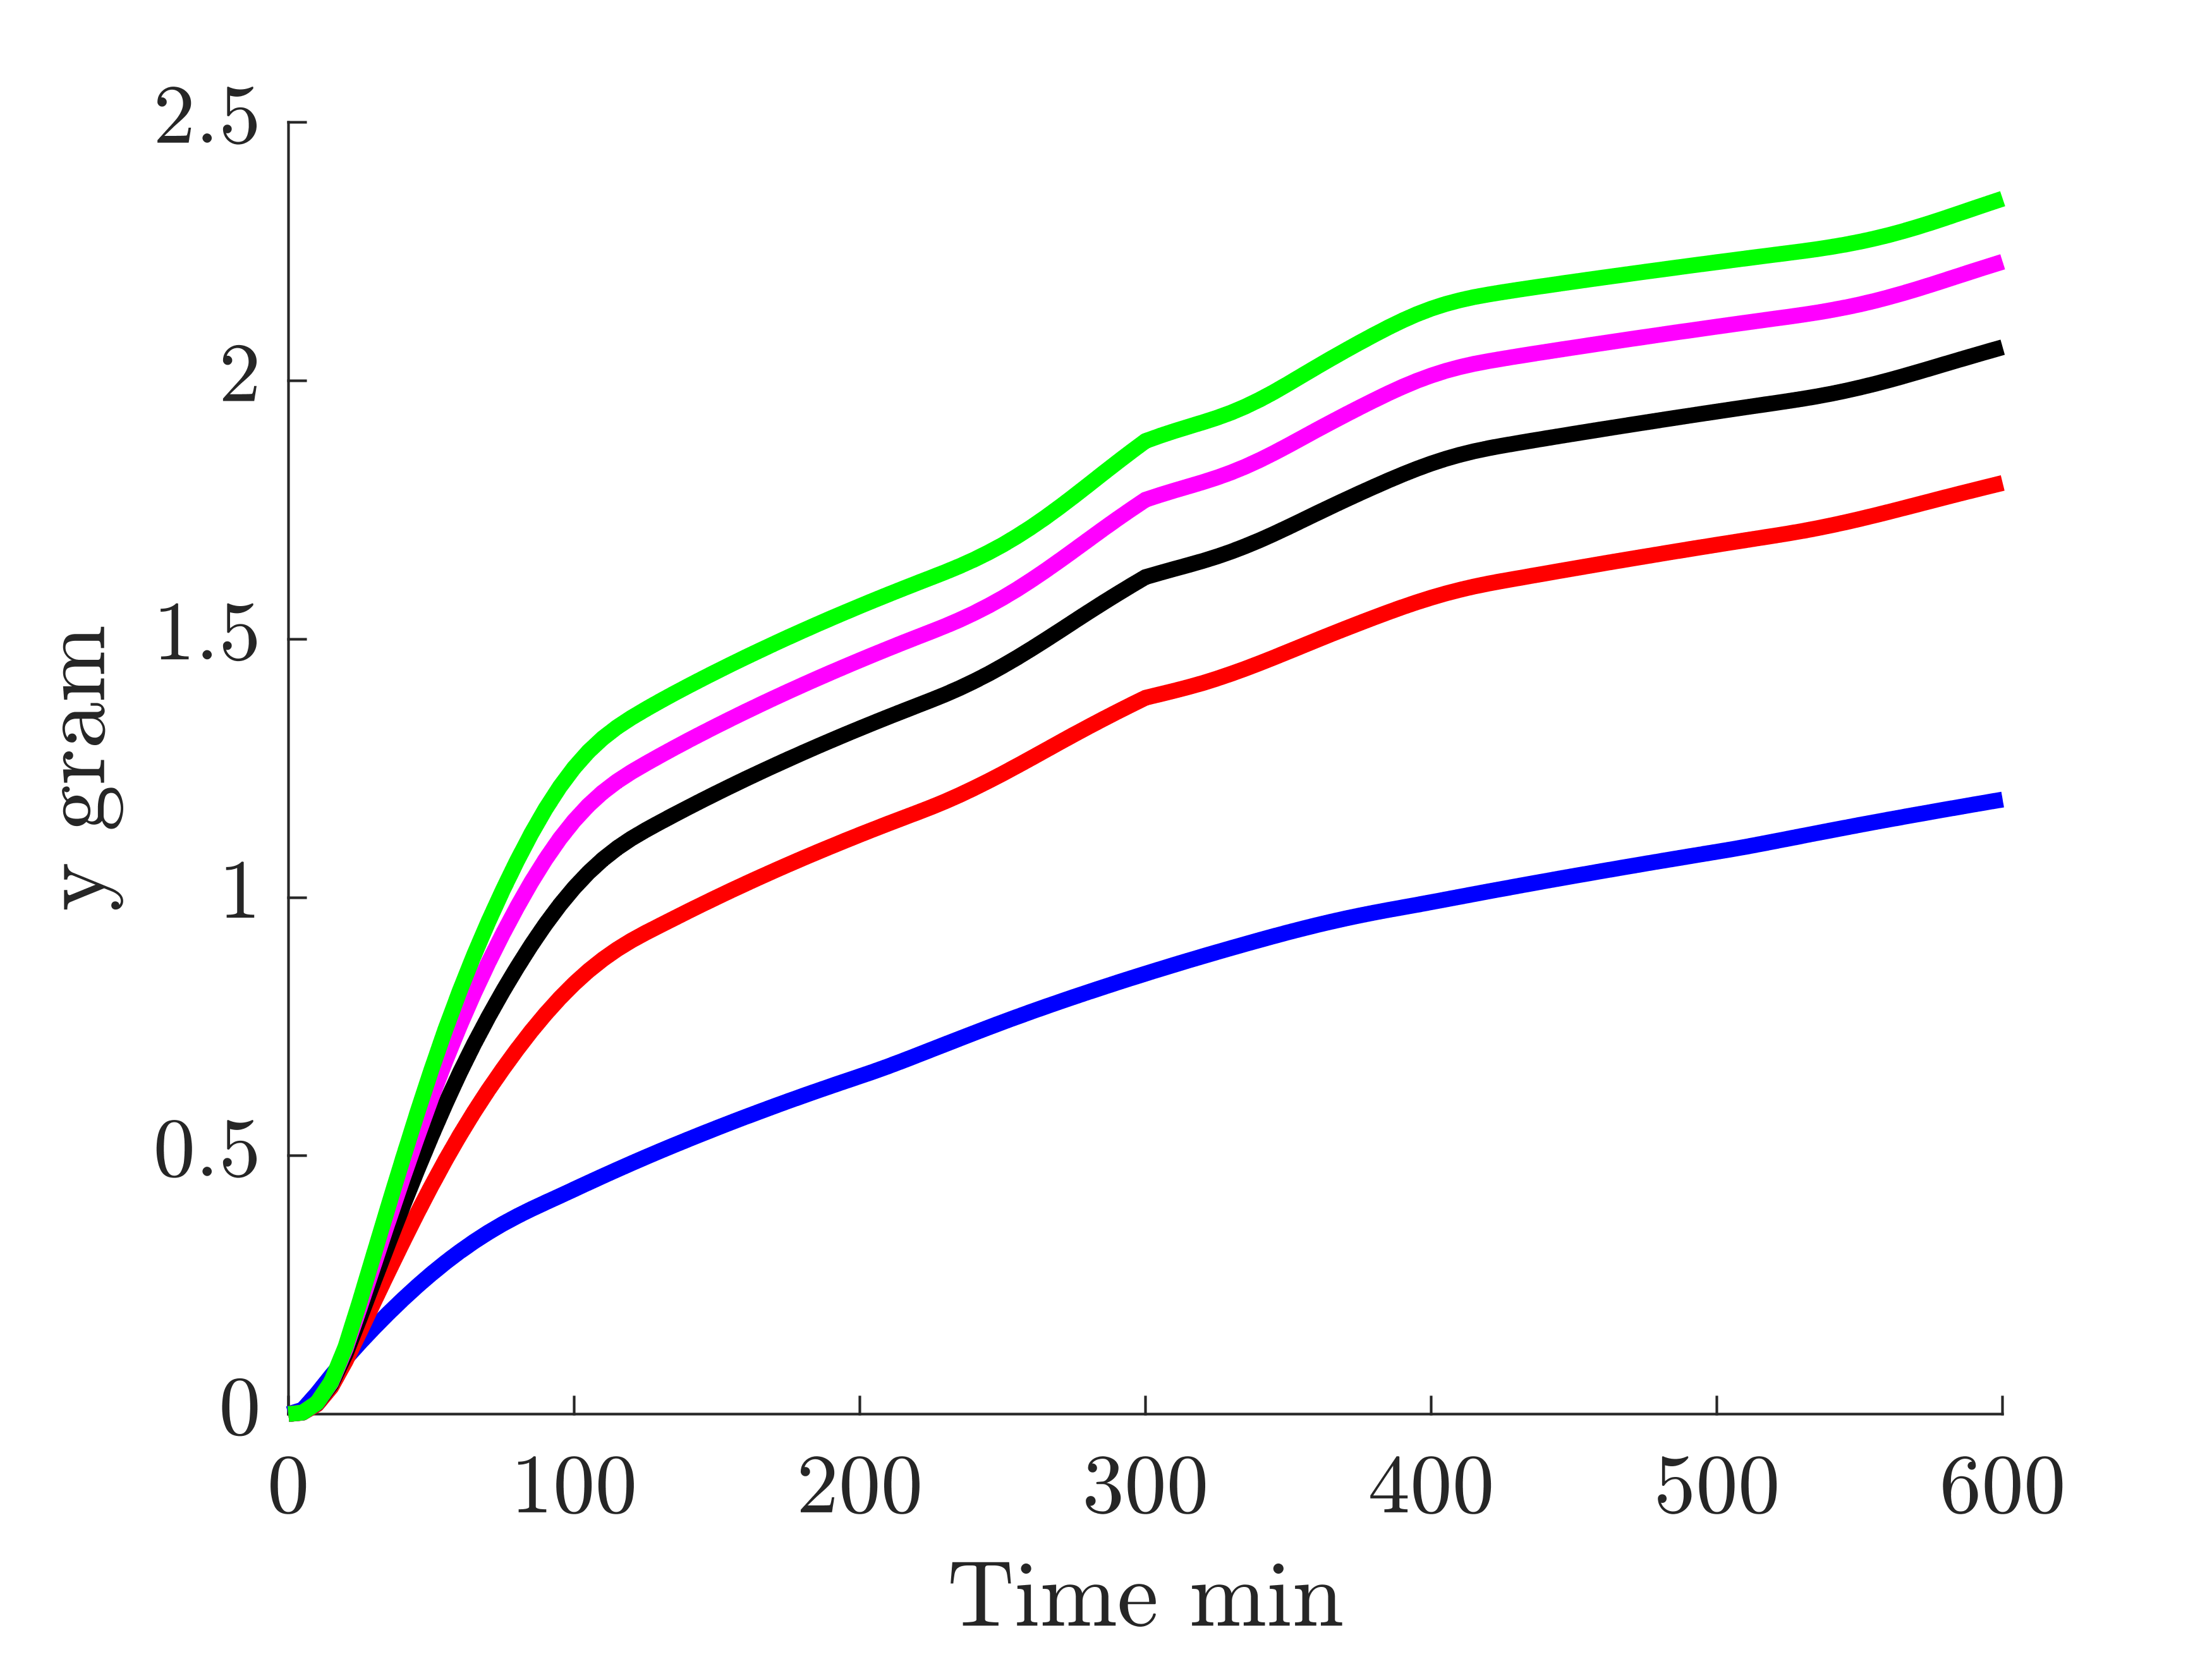
\includegraphics[width=0.90\columnwidth]{Figures/Results/yield.png}	
				\caption{Optimal yield profiles}
				\label{fig:profiles_y}
			\end{subfigure}
			\caption{Results of the optimisation problem.}
		\end{figure}	
		
		Figure \ref{fig:profiles_T} shows the optimal profiles of the inlet temperature ($T^{in}$) for various pressure cases in the supercritical CO$_2$ extraction process. Initially, the $T^{in}$ remains constant at approximately $40~^\circ C$ for all pressures, indicating a stable starting condition for the system. The temperature decreases after about 300 min, but the exact time varies slightly depending on the pressure. This decline is rapid for lower pressures and gradual for higher pressures. The blue curve (100 bar) exhibits the sharpest temperature drop, while the green curve (200 bar) demonstrates a slower and more gradual decline. At lower pressures, the final temperature reaches the critical temperature and remains steady until the end of the batch. In contrast, the higher pressure cases result in a less significant temperature reduction. Moreover, the system does not reach steady operating conditions, as the inlet temperature profile does not flatten by the end of the process.
		
		Figure \ref{fig:profiles_y} depicts the predicted yield curves. A closer examination of the yield and scatter plots reveals that the most informative experiments do not necessarily correspond to those with the highest yield. When the D-optimality criterion is applied, the aim is to maximise the determinant of the Fisher information matrix across the experimental design space. This approach identifies conditions that amplify variations in observed responses, particularly in regions with high sensitivity to parameter changes. As a result, the yield curve may display a "wavy" pattern, characterised by oscillations rather than a smooth, monotonic trend. These fluctuations arise from increased multiple critical points - local maxima, minima or saddle points - on the response surface. By maximising the sum of determinants of the Fisher information matrix, the experimental design prioritises regions of high curvature, where the response changes sharply. 
		
		Alternatively, the D-optimality problem can be understood through the concept of Gaussian curvature. In this view, the experimental design shapes the parameter space of a model into a manifold with local geometry defined by the Fisher information matrix. The D-optimality condition maximises the determinant of this matrix, which geometrically corresponds to maximising the product of the principal curvatures of the manifold at a given point. This determinant is directly proportional to the Gaussian curvature, linking experimental design to the geometry of the parameter space. The determinant of the Fisher information matrix can be interpreted as a measure of the "volume element" on the parameter manifold, with higher values indicating regions of greater local curvature. By maximising this determinant, the parameter manifold is locally as curved as possible, which explains the wavy behaviour of the yield curves.
		
		To the authors knowledge, model-based dynamic design of experiments has not previously been applied to supercritical extraction, hence the authors cannot directly compare the obtained results against the literature. Nevertheless, some researchers proposed running an extraction process under dynamically changing operating conditions. For instance, \citet{Simandi1998} proposed a fractionated extraction of oregano with a stepwise increase in pressure (80, 120, 200, and 300 bar). As a result, the obtained yield curve exhibits non-monotonic patterns. \citet{Hiraga2025} suggested a pressure swing CO$_2$ extraction for the decaffeination of green coffee beans. The authors varied the pressure up and down during the operation, achieving a high degree of decaffeination with a reduced CO$_2$ supply. As a result, nearly 100\% decaffeination was achieved at 353 K and 30 MPa, using 80\% of the CO$_2$ supply compared to the case of constant pressure operation. Some of the extraction yield plots presented by \citet{Hiraga2025} are characterised by non-monotonic behaviour. It can be concluded that non-monotonic extraction curves have been reported in the literature.
		
		The results and observations discussed in this article are local and should be considered valid only for the model presented in \citet{Sliczniuk2024}. Although general conclusions about the curvature of the yield curve are independent of the process model, a completely different set of control profiles should be expected if the same technique is applied to a different model. Such strong dependence on the model is one of the most significant limitations of this work. Moreover, the model predicts the data set in a region which has not been validated during previous experiments. This leaves room for model validation, while on the other hand, the obtained set of data points might differ from the predictions.
		
		\section{Conclusion} \label{CH: Conclusion}
		This paper introduces D-optimal experimental design (D-OED) as a model-based method for determining optimal	experimental procedures in chemical engineering problems. D-OED optimises an objective function, which can be geometrically	interpreted as minimising the volume of the uncertainty ellipsoid, thereby maximising the precision of parameter estimates. Compared to the classical formulation of D-OED, this work introduces a penalty term to the cost function to prevent unrealistic rapid changes in operating conditions, ensuring practical feasibility in experimental	implementation. The method is demonstrated through a case study on supercritical extraction, focusing on designing experiments	to improve the precision of the correlation for the diffusivity coefficient $D_i$. While the original experiments were conducted under constant operating conditions, this study explores dynamically changing operating conditions, highlighting the potential of D-OED solutions for both parameter estimation and model validation.
		
		The analysis was conducted for multiple pressure cases and the optimal mass flow rate profiles were similar across all instances. The inlet temperature profiles show different patterns, but all start with high temperature that decreases in	the second half of the batch. The resulting yield curves exhibit distinct wavy patterns, which can be explained through	the relationship between the Hessian matrix and the Gaussian curvature of a multi-variable function. The determinant of the Fisher information matrix, central to the D-optimality criterion, is proportional to the Gaussian curvature of the parameter manifold. This curvature reflects the system’s sensitivity to parameter changes and is maximised by the D-OED method. The observed wavy behaviour of the yield curves is thus a manifestation of the high-curvature regions identified by the optimisation, where the system’s response to experimental conditions is most informative.
		
		Further analysis of the yield curves and scatter plots reveals that the informativeness of experiments varies significantly across different operating conditions. This variation depends on the physical properties of CO$_2$, which change	significantly around the critical point. Consequently, it is concluded that operating conditions must be carefully selected for the specific regime of interest to maximise the information gained. This observation emphasises the importance of aligning experimental strategies with the system’s underlying physical properties and model structure.

% ===================================================
% Bibliography
% ===================================================
%% Loading bibliography style file
%\clearpage
%\newpage
%\bibliographystyle{model1-num-names}
\bibliographystyle{unsrtnat}
\bibliography{mybibfile}

%\clearpage \appendix \label{appendix}
%\section{Appendix} 
%\subfile{Sections/Qubic_EOS} \label{CH: EOS}
%\subsection{Cardano's Formula} \label{CH: Cardano}
%\subfile{Sections/Cardano}

%\clearpage
%\newpage

\nomenclature[A]{\(A\)}{Information matrix \nomunit{[-]}}
\nomenclature[A]{\(A\)}{Total cross-section of the bed \nomunit{$m^2$}}
\nomenclature[A]{\(A_f\)}{Cross-section of the bed occupied by the fluid \nomunit{$m^2$}}
\nomenclature[A]{\(B\)}{Pressure dependent parameter of P-R EoS \nomunit{$m^2$}}
\nomenclature[A]{\(B\)}{Weighted score vector \nomunit{[-]}}
\nomenclature[A]{\(C\)}{Weighted sum of squared deviations \nomunit{[-]}}
\nomenclature[A]{\(c_f\)}{Concentration of solute in the fluid phase \nomunit{kg/$m^3$}}
\nomenclature[A]{\(c_f^*\)}{Concentration of solute at the solid-fluid interface \nomunit{kg/$m^3$}}
\nomenclature[A]{\(c_{f0}\)}{Initial concentration of solute in the fluid phase \nomunit{kg/$m^3$}}
\nomenclature[A]{\(c_p\)}{Concentration of solute in the core of a pore \nomunit{kg/$m^3$}}
\nomenclature[A]{\(c_{pf}\)}{Concentration of solute at the pore opening \nomunit{kg/$m^3$}}
\nomenclature[A]{\(c_s\)}{Concentration of solute in the solid phase \nomunit{kg/$m^3$}}
\nomenclature[A]{\(c_s^*\)}{Concentration of solute at the solid-fluid interface \nomunit{kg/$m^3$}}
\nomenclature[A]{\(c_{s0}\)}{Initial concentration of solute in the solid phase \nomunit{kg/$m^3$}}
\nomenclature[A]{\(D_e^M\)}{Axial diffusion coefficient \nomunit{$m^2$/s}}
\nomenclature[A]{\(D_i\)}{Internal diffusion coefficient \nomunit{$m^2$/s}}
\nomenclature[A]{\(D_i^R\)}{Reference value of internal diffusion coefficient \nomunit{$m^2$/s}}
\nomenclature[A]{\(e\)}{Internal energy \nomunit{J/kg}}
\nomenclature[A]{\(F\)}{Mass flow rate \nomunit{kg/s}}
\nomenclature[A]{\(G\)}{Vector of discretized differential equations \nomunit{[-]}}
\nomenclature[A]{\(h\)}{Enthalpy \nomunit{kJ/kg}}
\nomenclature[A]{\(J\)}{Jacobian \nomunit{[-]}}
\nomenclature[A]{\(j\)}{Objective function \nomunit{[-]}}
\nomenclature[A]{\(k_m\)}{Mass partition coefficient \nomunit{[-]}}
\nomenclature[A]{\(k_p\)}{Volumetric partition coefficient \nomunit{[-]}}
\nomenclature[A]{\(L\)}{Length of the fixed bed \nomunit{m}}
\nomenclature[A]{\(l\)}{Characteristic dimension of particles \nomunit{m}}
\nomenclature[A]{\(n_\theta\)}{Number of analyzed parameters \nomunit{[-]}}
\nomenclature[A]{\(n_y\)}{Number of measurements \nomunit{[-]}}
\nomenclature[A]{\(N_z\)}{Number of discretized points in z-direction \nomunit{[-]}}
\nomenclature[A]{\(P\)}{Pressure \nomunit{bar}}
\nomenclature[A]{\(P_r\)}{Reduced pressure \nomunit{[-]}}
\nomenclature[A]{\(p\)}{Probability distribution model \nomunit{[-]}}
\nomenclature[A]{\(Q\)}{Weighting matrix \nomunit{[-]}}
\nomenclature[A]{\(Re\)}{Reynolds number \nomunit{[-]}}
\nomenclature[A]{\(r\)}{Particle radius \nomunit{m}}
\nomenclature[A]{\(r_e\)}{Mass transfer kinetic term \nomunit{kg/$m^3$/s}}
\nomenclature[A]{\(T\)}{Temperature \nomunit{K}}
\nomenclature[A]{\(T_{in}\)}{Inlet temperature \nomunit{K}}
\nomenclature[A]{\(T_{out}\)}{Outlet temperature \nomunit{K}}
\nomenclature[A]{\(T_r\)}{Reduced temperature \nomunit{[-]}}
\nomenclature[A]{\(t\)}{Time \nomunit{s}}
\nomenclature[A]{\(t_0\)}{Initial extraction time \nomunit{s}}
\nomenclature[A]{\(t_f\)}{Total extraction time \nomunit{s}}
\nomenclature[A]{\(u\)}{Superficial velocity \nomunit{m/s}}
\nomenclature[A]{\(v\)}{Linear velocity \nomunit{m/s}}
\nomenclature[A]{\(x\)}{State vector \nomunit{[-]}}
\nomenclature[A]{\(Y\)}{Yield measurement \nomunit{g}}
\nomenclature[A]{\(y\)}{Predicted extraction yield \nomunit{g}}
\nomenclature[A]{\(Z\)}{Compressibility factor \nomunit{[-]}}
\nomenclature[A]{\(z\)}{Spatial direction \nomunit{m}}

% Non-latin symbols
\nomenclature[B]{\(\mathcal{F}\)}{Fisher information \nomunit{[-]}}
\nomenclature[B]{\(\mathcal{R}\)}{Control cost matrix \nomunit{[-]}}

% Greek symbols
\nomenclature[C]{\(\alpha\)}{Temperature-dependent function in the P-R EoS \nomunit{[-]}}
\nomenclature[C]{\(\Delta_\theta\)}{Residual term of the parameters \nomunit{g}}
\nomenclature[C]{\(\Delta_y\)}{Residual term of the measurement error \nomunit{g}}
\nomenclature[C]{\(\epsilon\)}{Unobservable error \nomunit{g}}
\nomenclature[C]{\(\gamma\)}{Decaying function \nomunit{[-]}}
\nomenclature[C]{\(\kappa\)}{Quadratic function of the acentric factor \nomunit{[-]}}
\nomenclature[C]{\(\mu\)}{Sphericity coefficient \nomunit{[-]}}
\nomenclature[C]{\(\phi\)}{Bed porosity \nomunit{[-]}}
\nomenclature[C]{\(\pi\)}{Probability density \nomunit{[-]}}
\nomenclature[C]{\(\rho_f\)}{Fluid density \nomunit{kg/$m^3$}}
\nomenclature[C]{\(\rho_s\)}{Bulk density of solid \nomunit{kg/$m^3$}}
\nomenclature[C]{\(\Sigma\)}{Covariance matrix \nomunit{[-]}}
\nomenclature[C]{\(\Sigma_\theta\)}{Parameter uncertainty matrix \nomunit{[-]}}
\nomenclature[C]{\(\Sigma_Y\)}{Measurement covariance matrix \nomunit{[-]}}
\nomenclature[C]{\(\sigma\)}{Standard deviation \nomunit{[-]}}
\nomenclature[C]{\(\Theta\)}{Parameter space \nomunit{[-]}}
\nomenclature[C]{\(\theta\)}{Vector of analysed parameters \nomunit{[-]}}
\nomenclature[C]{\(\Upsilon\)}{Decay coefficient \nomunit{[-]}}
\nomenclature[C]{\(\varkappa\)}{An arbitrary function of \(\mathcal{A}\)}
\nomenclature[C]{\(\Xi\)}{Matrix of experimental conditions \nomunit{[-]}}
\nomenclature[C]{\(\xi\)}{Vector of experimental conditions \nomunit{[-]}}

% Abbreviations
\nomenclature[D]{BIC}{Broke-and-Intact Cell model}
\nomenclature[D]{DoE}{Design of Experiment}
\nomenclature[D]{HBD}{Hot Ball Diffusion}
\nomenclature[D]{m-DoE}{Model-based Design of Experiment}
\nomenclature[D]{P-R EoS}{Peng-Robinson Equation of State}
\nomenclature[D]{SC}{Shrinking Core}
\nomenclature[D]{SFE}{Supercritical Fluid Extraction}
\printnomenclature

\clearpage
\onecolumn
\appendix
\section{Literature Review} \label{CH: Literature}
Table \ref{fig: SFE_Literature} provides a list of studies on SFE including the modelling part presented from 2014 onwards

\begin{table*}[h!]
	\centering
	\resizebox{\textwidth}{!}{%
	\begin{tabular}{|p{2.5cm}|p{2cm}|p{1.75cm}|p{4.5cm}|p{1.5cm}|p{1.5cm}|p{3cm}|}
		\hline
		\textbf{Reference} & \textbf{Substrate} & \textbf{Solvent} & \textbf{Model} & \textbf{T (°C)} & \textbf{P (MPa)} & \textbf{Flow-rate of CO$_2$} \\
		\hline
		\citet{Botelho2015} & Black sesame seed & CO$_2$ & BIC (\citet{Sovova1994}) \newline Local adsorption equilibrium model (\citet{Goto1993}) &  40, 60 & 20-40 & 5.9$\times 10^{-5}$ [kg/s]\\ \hline
		\citet{Melo2014} & Eucalyptus globulus bark & CO$_2$, \newline Co-solvent: ethanol & Diffusion model (\citet{Crank1975}) \newline \citet{Brunner1994} \newline Desorption model (\citet{Cocero2001}) \newline SSP model (\citet{Gaspar2003})&  40 & 20 & 2.78$\times 10^{-3}$ [kg/s]\\ \hline
		\citet{Liu2014} & Calycopteris floribunda leaves & CO$_2$, \newline Co-solvent: ethanol & BIC (\citet{Sovova1994}) \newline Diffusion model (\citet{Crank1975}) &  30–50 & 10-30 & 4.17$\times 10^{-4}$ [kg/s]\\ \hline
		\citet{Tomita2014} & Rice bran & CO$_2$ & Partitioning coefficient model (\citet{Kubatova2002}) & 40–80 & 20-40 & 0.17-1.5$\times 10^{-4}$ [L/s]\\ \hline
		\citet{Kupski2017} & Hop pellet & CO$_2$ & BIC (\citet{Sovova1994}) \newline \citet{Reverchon1996} &  35-55 & 10-20 & 3.25$\times 10^{-5}$ [kg/s]\\ \hline
		\citet{Pavlic2017} & Sage & CO$_2$ & \citet{Reverchon1996} \newline  \citet{Brunner1994} \newline \citet{Kandiah1990} &  40-60 & 10-30 & 5.56-11.1$\times 10^{-5}$ [kg/s]\\ \hline
		\citet{Sartori2017} & Banana & CO$_2$ & \citet{Sovova1994} \newline  \citet{Reverchon1994} \newline \citet{Esquivel1999} &  40-80 & 20-50 & 1.01$\times 10^{-4}$ [L/s]\\ \hline
		\citet{Hall2018} & Papaya seeds & CO$_2$ & \citet{Sovova1994} \newline  \citet{Goto1993} \newline \citet{Esquivel1999} &  40 & 15-30 & 6.11-19.4$\times 10^{-5}$ [kg/s]\\ \hline
		\citet{Putra2018} & Peanut skin & CO$_2$, \newline Co-solvent: ethanol & \citet{Brunner1994} \newline \citet{Esquivel1999} &  40-70  & 10-30 & 5$\times 10^{-5}$ [L/s]\\ \hline
		\citet{Putra2018} & Wheat germ & CO$_2$ & \citet{Brunner1994} \newline \citet{Esquivel1999} \newline \citet{Kandiah1990} \newline \citet{Reverchon1994} &  40-60  & 25-35 & 0.56 - 1.11 $\times 10^{-4}$ [kg/s]\\ \hline
		\citet{Pavlic2020} & Raspberry seed & CO$_2$ & \citet{Brunner1994} \newline \citet{Esquivel1999} \newline \citet{Kandiah1990} \newline \citet{Reverchon1994} &  40-60  & 25-35 & 0.56 - 1.11 $\times 10^{-4}$ [kg/s]\\ \hline
		\citet{Priyanka2020} & Carrot seed & CO$_2$, \newline Co-solvent: ethanol & BIC (\citet{Sovova1994}) \newline \citet{Reverchon1997} &  50-70  & 20-40 & 0.83 - 2.5 $\times 10^{-4}$ [kg/s]\\ \hline
		\citet{Casas2021} & Acacia dealbata - flowers & CO$_2$, \newline Co-solvent: ethanol & \citet{Esquivel1999} \newline \citet{Sovova1994} &  35-55  & 10-35 & 4.17 $\times 10^{-4}$ [kg/s]\\ \hline
		\citet{Acosta2014} & Wood (\textit{Mezilaurus itauba}) & CO$_2$, \newline Co-solvent: ethanol (2\%, 5\%, 8\%) & BIC(\citet{Sovova1994}) &  38-52  & 8-22 & 5 $\times 10^{-5}$ [L/s]\\ \hline
		\citet{Zekovic2014} & \textit{Ocimum basilicum L.} & CO$_2$ & \citet{Brunner1994} \newline \citet{Kandiah1990} \newline \citet{Esquivel1999} &  40-60  & 10-30 & 2.71 $\times 10^{-2}$ [L/s]\\ \hline
	\end{tabular} }
	\caption{SFE studies encompassing modeling part}
	\label{fig: SFE_Literature}
\end{table*}

\end{document}